\documentclass[conference]{IEEEtran}
\IEEEoverridecommandlockouts
\usepackage{cite}
\usepackage{amsmath,amssymb,amsfonts}
%\usepackage{algorithmic}
\usepackage{graphicx}
\usepackage{textcomp}
\usepackage{xcolor}
\usepackage{booktabs}
\usepackage{multirow}
\usepackage{array}
\usepackage{tabularx}
\usepackage{float}
\usepackage{url}
\usepackage{tikz}
\usetikzlibrary{shapes.geometric, arrows.meta, positioning, fit, calc}
%\usepackage{pgfplots}
%\pgfplotsset{compat=1.18}
\usepackage[font=small]{caption}
%\usepackage{balance}

\def\BibTeX{{\rm B\kern-.05em{\sc i\kern-.025em b}\kern-.08em
    T\kern-.1667em\lower.7ex\hbox{E}\kern-.125emX}}

\begin{document}

\title{AI-Based Accident Hotspot Prediction and Severity Classification Using DBSCAN Spatial Clustering and Random Forest}

\author{%
\begin{tabular}{cc}
  \begin{tabular}[t]{c}
    {1\textsuperscript{st} Anuhya Valluri}\\[0.4ex]
    \textit{School of Computer Applications}\\
    \textit{Lovely Professional University}\\
    Phagwara, Punjab, India
  \end{tabular}
  \qquad\qquad
  &
  \qquad\qquad
  \begin{tabular}[t]{c}
    {2\textsuperscript{nd} Mehak}\\[0.4ex]
    \textit{School of Computer Applications}\\
    \textit{Lovely Professional University}\\
    Phagwara, Punjab, India
  \end{tabular}
  \\[3ex]
  \noalign{\vspace{3ex}}
  \begin{tabular}[t]{c}
    {3\textsuperscript{rd} Kashik Kumar}\\[0.4ex]
    \textit{School of Computer Applications}\\
    \textit{Lovely Professional University}\\
    Phagwara, Punjab, India
  \end{tabular}
  \qquad\qquad
  &
  \qquad\qquad
  \begin{tabular}[t]{c}
    {4\textsuperscript{th} Brojendro Ningthoujam}\\[0.4ex]
    \textit{School of Computer Applications}\\
    \textit{Lovely Professional University}\\
    Phagwara, Punjab, India
  \end{tabular}
\end{tabular}
}

\maketitle
\vspace{-1em}

\begin{abstract}
Road traffic accidents remain a major public safety problem in India, where more than 150,000 fatalities are reported each year. This paper presents an integrated pipeline that combines DBSCAN spatial clustering with Random Forest classification to identify accident black spots and estimate accident severity. The study uses 12,316 Indian road accident records and 17 engineered features. DBSCAN with haversine distance and $\varepsilon = 0.045$ radians identifies 9 accident clusters. The Random Forest model, trained with 200 estimators and balanced class weighting, reaches 84.66\% test accuracy and a weighted F1-score of 0.7793. Five-fold stratified cross-validation gives a mean accuracy of 84.76\%. A composite Accident Risk Index (ARI) combines severity, density, and environmental factors using weights derived from model feature importances. The resulting risk map separates clusters into Low, Moderate, and Severe tiers, with hour of day, cause of accident, and day of week emerging as the most informative predictors. The workflow is exposed through a Flask REST API.
\end{abstract}

\begin{IEEEkeywords}
accident hotspot, DBSCAN, Random Forest, severity prediction, spatial clustering, accident risk index, road safety
\end{IEEEkeywords}

\section{Introduction}

India accounts for roughly 11\% of global road accident fatalities, despite having only about 1\% of the world's registered vehicles \cite{b1}. The Ministry of Road Transport and Highways reported 461,312 road accidents and 168,491 deaths in 2022, which amounts to roughly 462 fatalities per day \cite{b2}. These numbers have remained stubbornly high for over a decade, and the economic cost is estimated at 3--5\% of India's GDP each year \cite{b3}.

Most accident management systems used in Indian cities are reactive. Crashes are documented, summarized later, and only then considered for intervention. That delay makes it harder to act on emerging black spots. A more useful workflow would detect spatial clusters early and estimate which conditions are linked with more severe outcomes, so authorities can prioritize limited resources.

This paper builds that workflow and makes three contributions:

\begin{enumerate}
\item A spatial clustering pipeline using DBSCAN with haversine distance that identifies 9 accident black spots from 12,316 geocoded Indian road accident records, without requiring pre-specification of cluster count.

\item A Random Forest classification model that predicts accident severity (Slight, Serious, or Fatal) using 17 features including the cluster membership itself, achieving 84.66\% accuracy on the test set and 84.76\% under five-fold cross-validation.

\item A composite Accident Risk Index (ARI) that merges severity, accident density, and environmental conditions into a single score per cluster, with weights derived from the Random Forest's own feature importances rather than set arbitrarily.
\end{enumerate}

The dataset is publicly available on Kaggle and includes records from different road types, weather conditions, and driver groups. Because the source data stores area categories rather than GPS points, those categories are geocoded to representative Indian city coordinates with controlled spatial jitter.

\section{Review of Literature}

Road accident research usually focuses on two problems: locating high-risk areas and predicting severity. This section keeps only the studies most relevant to the pipeline used here.

\subsection{Spatial analysis of accident locations}

GIS and spatial statistics have long been used for hotspot identification. Anderson \cite{b4} mapped crash concentrations with kernel density estimation, while Kumar and Toshniwal \cite{b6} showed that DBSCAN works well for Indian accident data because it does not require a pre-set number of clusters. Prasannakumar et al. \cite{b8} also reported that spatial clustering helps isolate the road segments carrying a disproportionate share of crashes.

\subsection{Machine learning for severity prediction}

Machine learning models have also been used for severity prediction. Abdel-Aty and Abdelwahab \cite{b9} showed early on that nonlinear models can outperform traditional regression. Random Forest remains a common choice; Jiang et al. \cite{b10} reported useful results on highway data, and Zong et al. \cite{b11} found that temporal variables repeatedly ranked near the top. Even so, class imbalance remains a central problem, especially for fatal crashes, and oversampling methods such as SMOTE are still widely used \cite{b14}.

\subsection{Combined spatial and predictive approaches}

Only a small number of studies combine spatial clustering with severity prediction in one workflow. Bao et al. \cite{b16} included spatiotemporal grouping before prediction, while Saha et al. \cite{b18} used a weighted severity index for black-spot analysis. Still, clustering, prediction, and risk scoring are often treated as separate tasks.

\section{Research Gap}

Three gaps motivate this work: cluster membership is often not used inside the severity model, many risk indices still depend on manual weighting, and multi-city Indian studies remain limited. This paper addresses those issues by feeding DBSCAN cluster IDs into the Random Forest model and deriving ARI weights from model importances.

\section{Methodology}

This section summarizes the main stages of the pipeline: data preparation, spatial clustering, severity classification, and risk scoring. Fig.~\ref{fig:architecture} shows the overall workflow.

\subsection{Dataset}

The dataset used in this study is the ``Road Accident Severity in India'' dataset, publicly available on Kaggle \cite{b19}. It contains 12,316 accident records with 37 raw columns covering accident circumstances, road conditions, vehicle information, and driver characteristics. The target variable is Accident\_severity, which takes three values: Slight Injury, Serious Injury, and Fatal Injury (mapped to numeric labels 1, 2, and 3 respectively).

Table~\ref{tab:dataset_overview} summarizes the key properties of the dataset after preprocessing.

\begin{table}[htbp]
\caption{Dataset Overview}
\begin{center}
\begin{tabular}{ll}
\toprule
\textbf{Property} & \textbf{Value} \\
\midrule
Total records & 12,316 \\
Features used (after engineering) & 17 \\
Severity classes & 3 \\
Unique area categories & 13 \\
Latitude range & 12.9386 -- 28.6345 \\
Longitude range & 72.5442 -- 88.3604 \\
\bottomrule
\end{tabular}
\label{tab:dataset_overview}
\end{center}
\end{table}

The severity distribution is heavily imbalanced, as shown in Table~\ref{tab:severity_dist}. Slight injuries account for 84.56\% of all records, while fatal injuries make up just 1.28\%. This imbalance directly affects classifier training and evaluation, a point we return to in Section~V.

\begin{table}[htbp]
\caption{Severity Class Distribution}
\begin{center}
\begin{tabular}{lrr}
\toprule
\textbf{Severity} & \textbf{Count} & \textbf{Percentage} \\
\midrule
Slight Injury & 10,415 & 84.56\% \\
Serious Injury & 1,743 & 14.15\% \\
Fatal Injury & 158 & 1.28\% \\
\midrule
Total & 12,316 & 100.00\% \\
\bottomrule
\end{tabular}
\label{tab:severity_dist}
\end{center}
\end{table}

\subsection{Data preprocessing}

\textbf{Geocoding.} The original dataset does not contain latitude and longitude fields. Instead, it contains an Area\_accident\_occured column with categorical values like ``Office areas'', ``Market areas'', and ``School areas''. These categories are mapped to representative coordinates of major Indian cities, and random spatial jitter of 2--8~km is applied to simulate within-city variation.

\textbf{Temporal feature engineering.} The Time column is parsed to extract the hour of day (0--23). The Day\_of\_week field is mapped to numeric values (0 = Monday through 6 = Sunday). A binary Is\_Night variable is derived from Light\_conditions, taking the value 1 when lighting conditions indicate darkness.

\textbf{Weather binning.} The Weather\_conditions column, which contains many fine-grained categories, is consolidated into six groups: Clear, Rain, Fog, Snow, Wind, and Other. This reduces sparsity while preserving the most safety-relevant weather distinctions.

\textbf{Categorical encoding.} Fifteen categorical features are transformed using label encoding. The encoders are serialized for later prediction.

\textbf{Missing value handling.} Missing categorical values are filled with ``Unknown'' before encoding. No records are dropped during preprocessing.

\subsection{System architecture}

Raw data passes through preprocessing into two branches: EDA for descriptive analysis and DBSCAN for spatial clustering. Cluster IDs are then appended to the feature matrix used by the Random Forest classifier. Model outputs and feature importances are finally used to compute ARI scores for each cluster.

\begin{figure}[htbp]
\centering
\resizebox{\columnwidth}{!}{%
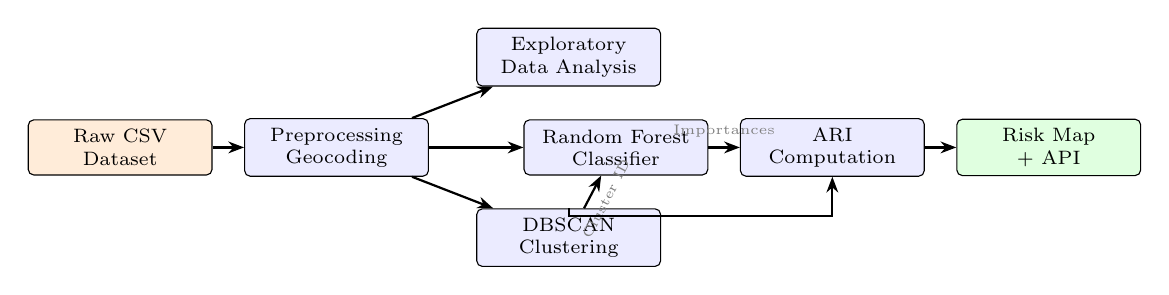
\begin{tikzpicture}[
    node distance=0.6cm and 0.4cm,
    block/.style={rectangle, draw, fill=blue!8, text width=2.1cm, minimum height=0.7cm, align=center, font=\scriptsize, rounded corners=2pt},
    arrow/.style={-{Stealth[length=2mm]}, thick},
    label/.style={font=\tiny, text=gray}
]
\node[block, fill=orange!15] (data) {Raw CSV\\Dataset};
\node[block, right=of data] (preprocess) {Preprocessing\\Geocoding};
\node[block, above right=0.4cm and 0.6cm of preprocess] (eda) {Exploratory\\Data Analysis};
\node[block, below right=0.4cm and 0.6cm of preprocess] (dbscan) {DBSCAN\\Clustering};
\node[block, right=1.2cm of preprocess] (rf) {Random Forest\\Classifier};
\node[block, right=of rf] (ari) {ARI\\Computation};
\node[block, right=of ari, fill=green!12] (riskmap) {Risk Map\\+ API};

\draw[arrow] (data) -- (preprocess);
\draw[arrow] (preprocess) -- (eda);
\draw[arrow] (preprocess) -- (dbscan);
\draw[arrow] (dbscan) -- node[label, below, sloped] {Cluster ID} (rf);
\draw[arrow] (preprocess) -- (rf);
\draw[arrow] (rf) -- node[label, above] {Importances} (ari);
\draw[arrow] (dbscan) |- ([yshift=-0.5cm]ari.south) -- (ari);
\draw[arrow] (ari) -- (riskmap);
\end{tikzpicture}
}
\caption{System architecture showing the pipeline from raw data to risk map output. DBSCAN cluster IDs are fed into the Random Forest as a spatial feature.}
\label{fig:architecture}
\end{figure}

\subsection{DBSCAN spatial clustering}

DBSCAN groups nearby points into dense regions and labels isolated points as outliers \cite{b20}. Unlike K-Means, it does not require the number of clusters in advance. For this study, the algorithm uses haversine distance on radian-transformed coordinates with ball-tree indexing for efficient neighbor search.

Two parameters control DBSCAN's behavior:

\begin{itemize}
\item \textbf{Epsilon ($\varepsilon$)}: the maximum distance between two points for them to be considered neighbors. Set to 0.045 radians, which corresponds to approximately 287~km ($\varepsilon \times R_{earth} = 0.045 \times 6371$~km).
\item \textbf{MinPts}: the minimum number of points required to form a dense region. Set to 15.
\end{itemize}

Table~\ref{tab:dbscan_params} lists the full DBSCAN configuration.

\begin{table}[htbp]
\caption{DBSCAN Clustering Configuration}
\begin{center}
\begin{tabular}{ll}
\toprule
\textbf{Parameter} & \textbf{Value} \\
\midrule
Algorithm & DBSCAN \\
Distance metric & Haversine \\
Epsilon ($\varepsilon$) & 0.045 radians ($\approx$287 km) \\
MinPts & 15 \\
Indexing structure & Ball tree \\
Clusters found & 9 \\
Noise points & 0 (0.0\%) \\
Clustered points & 12,316 (100\%) \\
\bottomrule
\end{tabular}
\label{tab:dbscan_params}
\end{center}
\end{table}

Each cluster is summarized by centroid, incident count, mean severity, and dominant weather condition. The cluster ID is then appended to the processed dataset as a classifier input.

\subsection{Random Forest classification}

Random Forest is an ensemble of decision trees trained on bootstrapped subsets of data \cite{b21}. The classifier uses the 17 features listed in Table~\ref{tab:features} to predict three severity classes. An 80/20 stratified split yields 9,852 training samples and 2,464 test samples.

\begin{table}[htbp]
\caption{Random Forest Hyperparameters}
\begin{center}
\begin{tabular}{ll}
\toprule
\textbf{Parameter} & \textbf{Value} \\
\midrule
Number of estimators & 200 \\
Maximum tree depth & 20 \\
Class weight & Balanced \\
Test set ratio & 0.2 (stratified) \\
Random state & 42 \\
Training samples & 9,852 \\
Test samples & 2,464 \\
\bottomrule
\end{tabular}
\label{tab:rf_params}
\end{center}
\end{table}

The ``balanced'' class weight setting scales each class inversely to its frequency in the training data, which gives more emphasis to the Serious and Fatal classes.

\begin{table}[htbp]
\caption{Feature Set for Classification (17 Features)}
\begin{center}
\footnotesize
\begin{tabular}{clc}
\toprule
\textbf{No.} & \textbf{Feature} & \textbf{Type} \\
\midrule
1 & Hour & Numeric \\
2 & DayOfWeek & Numeric \\
3 & Is\_Night & Binary \\
4 & Weather\_Binned\_Enc & Encoded \\
5 & Num\_Vehicles & Numeric \\
6 & Type\_of\_vehicle\_Enc & Encoded \\
7 & Road\_surface\_type\_Enc & Encoded \\
8 & Road\_surface\_conditions\_Enc & Encoded \\
9 & Light\_conditions\_Enc & Encoded \\
10 & Type\_of\_collision\_Enc & Encoded \\
11 & Cause\_of\_accident\_Enc & Encoded \\
12 & Road\_allignment\_Enc & Encoded \\
13 & Types\_of\_Junction\_Enc & Encoded \\
14 & Lanes\_or\_Medians\_Enc & Encoded \\
15 & Driving\_experience\_Enc & Encoded \\
16 & Age\_band\_of\_driver\_Enc & Encoded \\
17 & Cluster\_ID & Spatial \\
\bottomrule
\end{tabular}
\label{tab:features}
\end{center}
\end{table}

Feature 17 (Cluster\_ID) is the DBSCAN output from the previous stage, allowing the classifier to use spatial context alongside the remaining attributes.

\subsection{Accident Risk Index (ARI)}

The ARI provides a single composite score per cluster that combines three factors: severity, accident density, and environmental conditions. It is computed as:

\begin{equation}
\text{ARI} = W_1 \cdot S_{sev} + W_2 \cdot S_{dens} + W_3 \cdot S_{env}
\label{eq:ari}
\end{equation}

\noindent where:

\begin{itemize}
\item $S_{sev}$ is the severity score, computed by normalizing the mean predicted severity of each cluster to the [0, 1] range using min-max scaling.
\item $S_{dens}$ is the density score, computed as the ratio of each cluster's incident count to the maximum incident count across all clusters.
\item $S_{env}$ is the environmental score, assigned based on the dominant weather condition in each cluster using the mapping in Table~\ref{tab:env_scores}.
\end{itemize}

\begin{table}[htbp]
\caption{Environmental Risk Scores by Weather Condition}
\begin{center}
\begin{tabular}{lc}
\toprule
\textbf{Weather} & \textbf{Risk Score} \\
\midrule
Clear & 0.15 \\
Wind & 0.55 \\
Rain & 0.75 \\
Fog & 0.80 \\
Snow & 0.85 \\
Other & 0.50 \\
\bottomrule
\end{tabular}
\label{tab:env_scores}
\end{center}
\end{table}

The weights $W_1$, $W_2$, and $W_3$ are derived from Random Forest feature importances. Features are grouped into severity-related, density/spatial, and environmental categories and then normalized so that $W_1 + W_2 + W_3 = 1$. In this study, the derived weights are $W_1 = 0.534$, $W_2 = 0.401$, and $W_3 = 0.065$.

The ARI score is clipped to [0, 1] and mapped to four risk tiers:

\begin{equation}
\text{Risk Tier} = 
\begin{cases}
\text{Low} & \text{if } 0.0 \leq \text{ARI} < 0.3 \\
\text{Moderate} & \text{if } 0.3 \leq \text{ARI} < 0.5 \\
\text{Severe} & \text{if } 0.5 \leq \text{ARI} < 0.7 \\
\text{Critical} & \text{if } 0.7 \leq \text{ARI} \leq 1.0
\end{cases}
\label{eq:tiers}
\end{equation}

\subsection{Evaluation metrics}

The classification model is evaluated using accuracy, precision, recall, F1-score (both macro and weighted averages), Cohen's Kappa ($\kappa$), Matthews Correlation Coefficient (MCC), log loss, and ROC-AUC (one-vs-rest). Five-fold stratified cross-validation provides estimates of generalization performance. Cohen's Kappa and MCC are included because they account for class imbalance more honestly than raw accuracy does.

\section{Results and Discussion}

This section reports the results from EDA, DBSCAN clustering, Random Forest classification, and ARI scoring.

\subsection{Exploratory data analysis}

The severity distribution (Fig.~\ref{fig:severity_dist}) confirms strong class imbalance: 84.56\% of records are Slight injuries. This pattern is consistent with national accident reporting trends in India \cite{b2}.

\begin{figure}[htbp]
\centerline{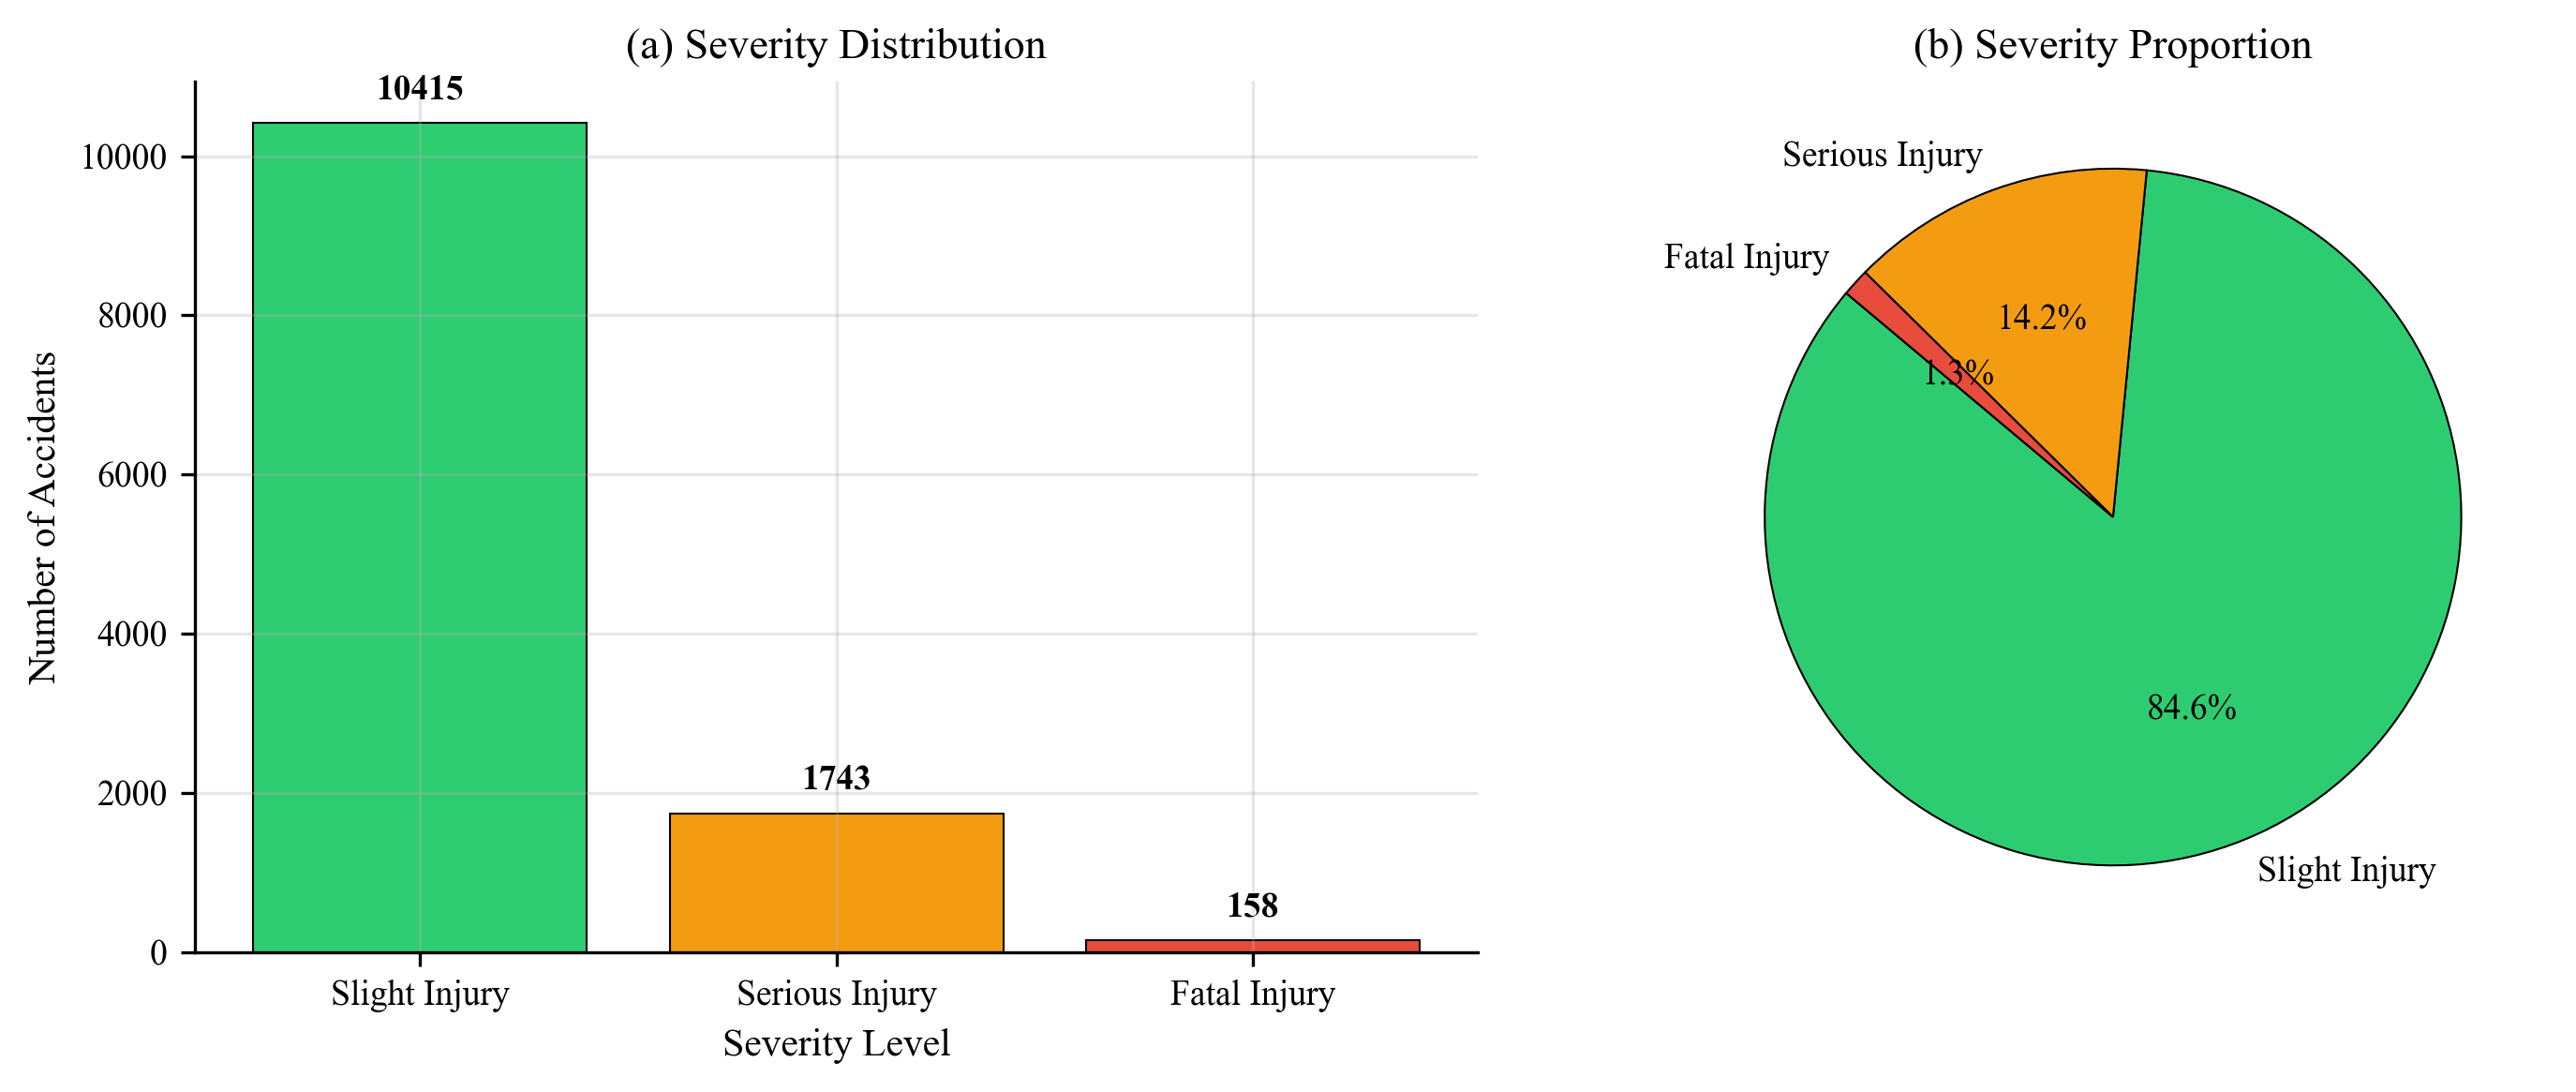
\includegraphics[width=\columnwidth]{figures/fig1_severity_distribution.png}}
\caption{Severity distribution shown as (a) bar chart with counts and (b) pie chart with percentages. Slight injuries dominate at 84.56\%.}
\label{fig:severity_dist}
\end{figure}

\textbf{Temporal patterns.} Fig.~\ref{fig:hourly} shows a bimodal pattern with peaks during morning and evening commute hours. Fig.~\ref{fig:daily} shows that Friday has the highest accident count, which matches earlier findings on end-of-week risk \cite{b11}.

\begin{figure}[htbp]
\centerline{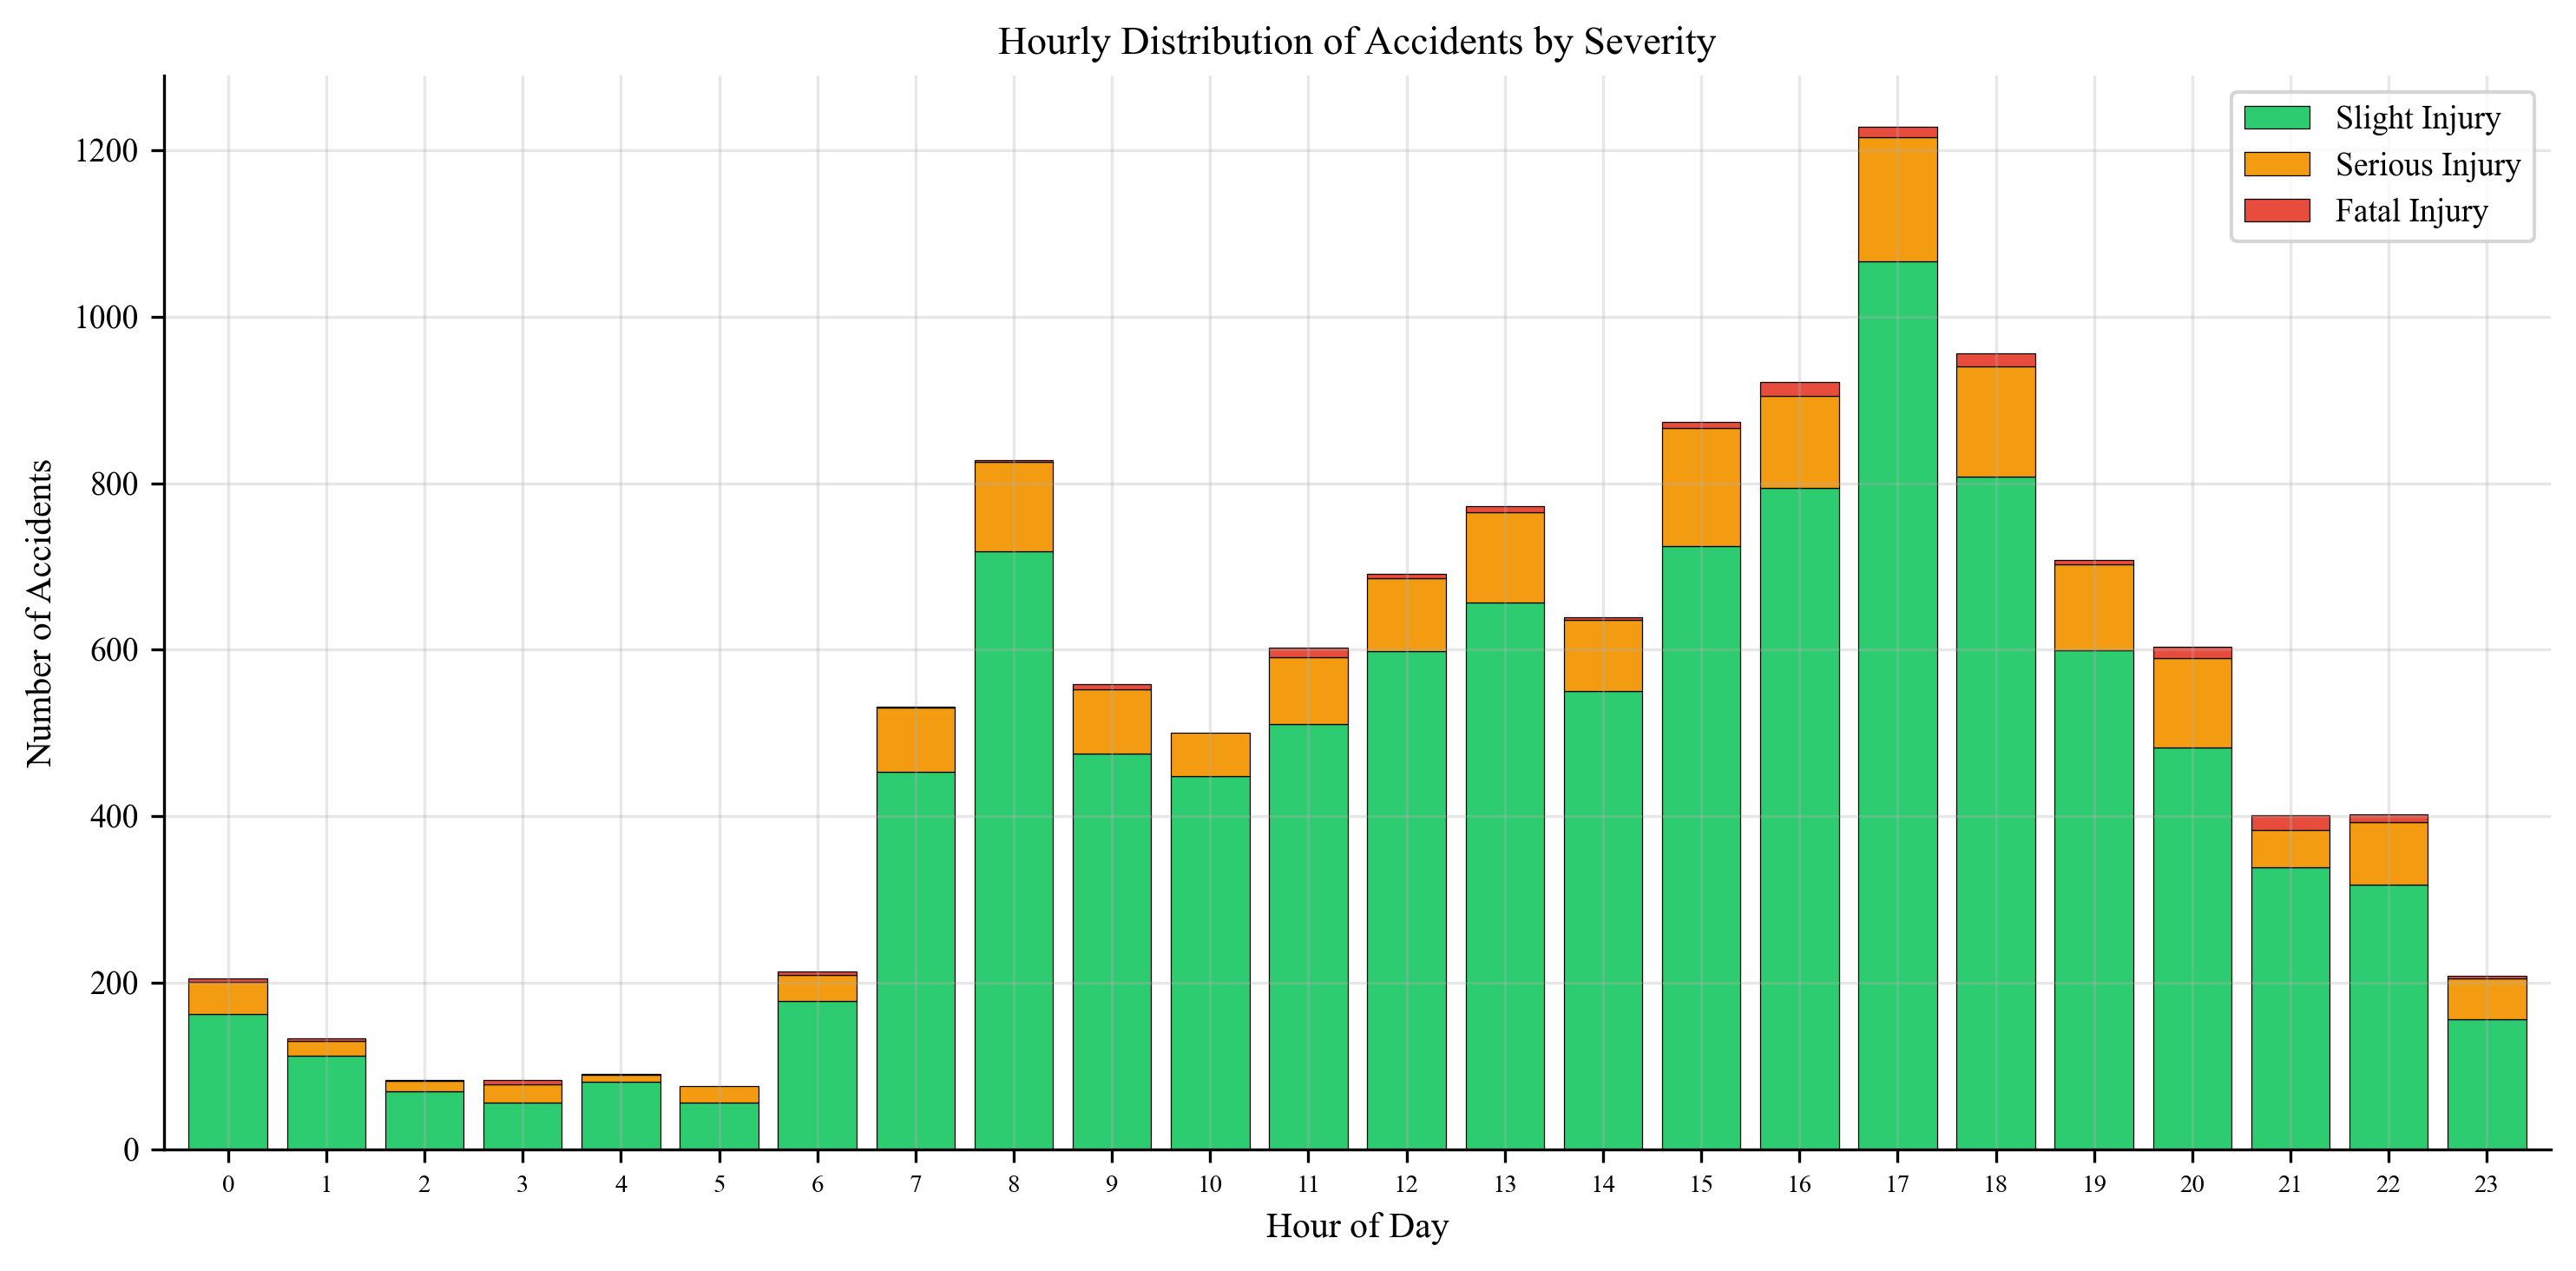
\includegraphics[width=\columnwidth]{figures/fig10_hourly_distribution.png}}
\caption{Accident frequency by hour of day. Peaks coincide with morning and evening commuting periods.}
\label{fig:hourly}
\end{figure}

\begin{figure}[htbp]
\centerline{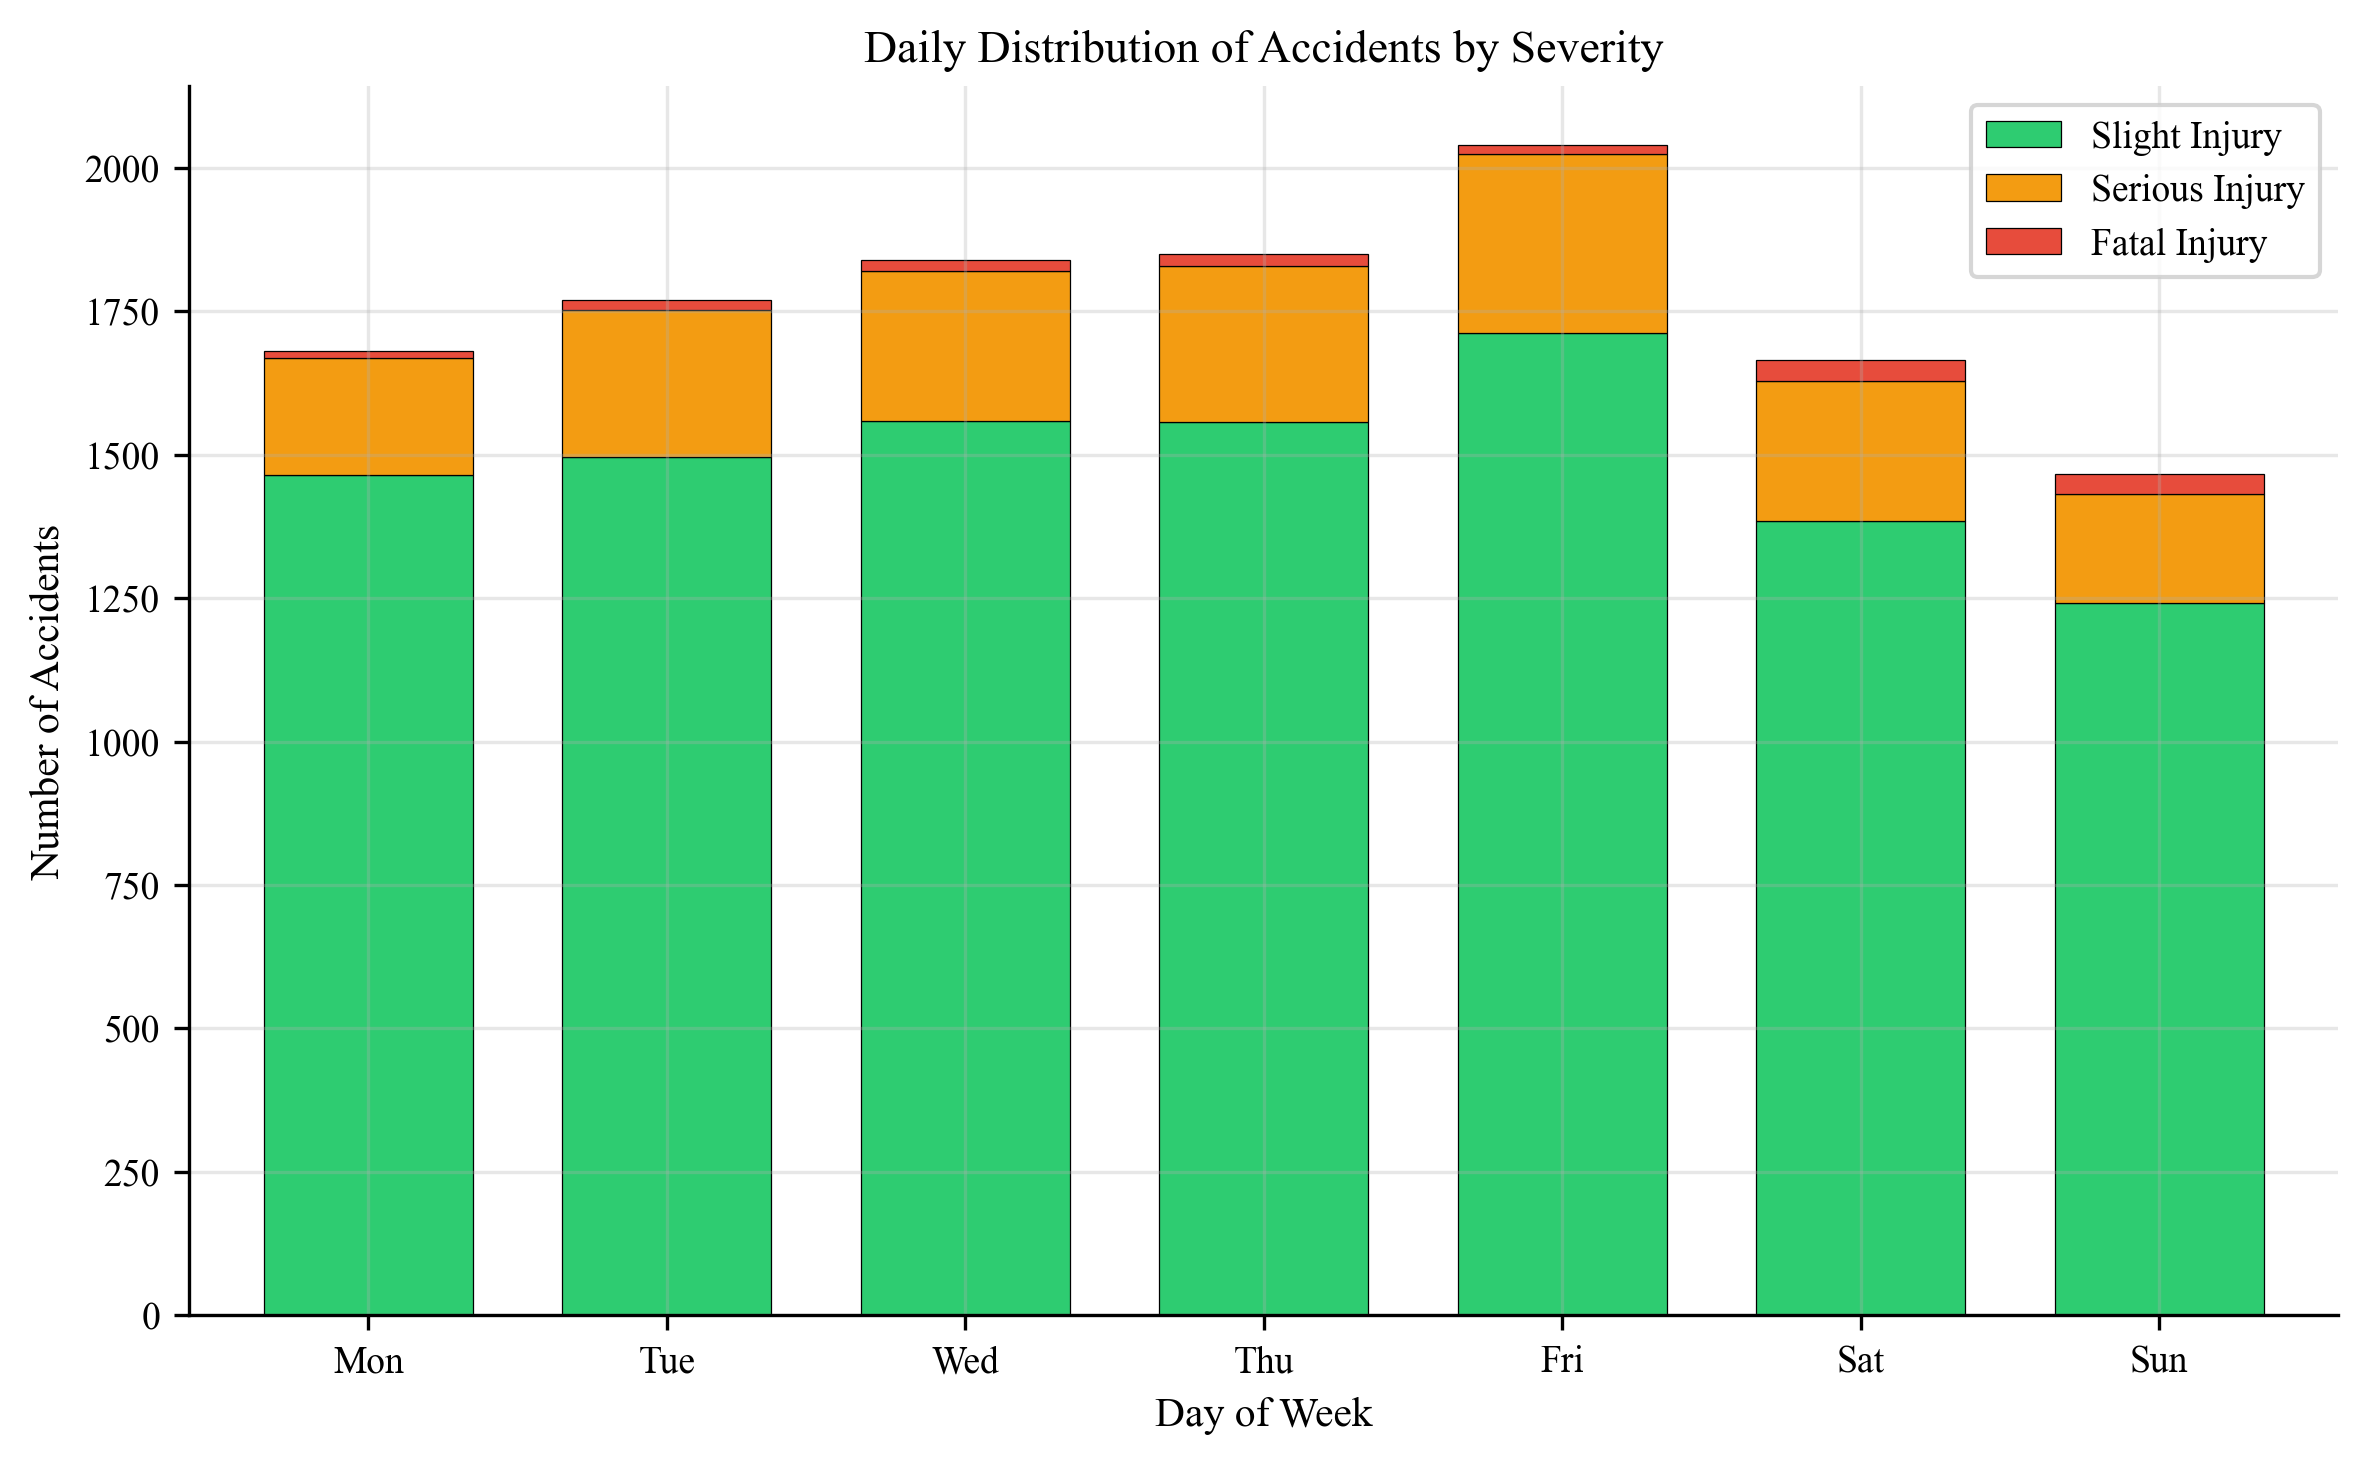
\includegraphics[width=\columnwidth]{figures/fig11_daily_distribution.png}}
\caption{Accident frequency by day of week. Friday shows the highest count.}
\label{fig:daily}
\end{figure}

\textbf{Weather and severity interaction.} Table~\ref{tab:weather_severity} shows that most accidents occur in clear weather, while rain is the second most common condition. Fig.~\ref{fig:weather_heatmap} visualizes this distribution.

\begin{table}[htbp]
\caption{Weather Condition vs. Severity Cross-tabulation}
\begin{center}
\footnotesize
\begin{tabular}{lrrrr}
\toprule
\textbf{Weather} & \textbf{Slight} & \textbf{Serious} & \textbf{Fatal} & \textbf{Total} \\
\midrule
Clear & 8,571 & 1,482 & 135 & 10,188 \\
Rain & 1,150 & 158 & 23 & 1,331 \\
Other & 547 & 81 & 0 & 628 \\
Wind & 82 & 16 & 0 & 98 \\
Snow & 56 & 5 & 0 & 61 \\
Fog & 9 & 1 & 0 & 10 \\
\midrule
Total & 10,415 & 1,743 & 158 & 12,316 \\
\bottomrule
\end{tabular}
\label{tab:weather_severity}
\end{center}
\end{table}

\begin{figure}[htbp]
\centerline{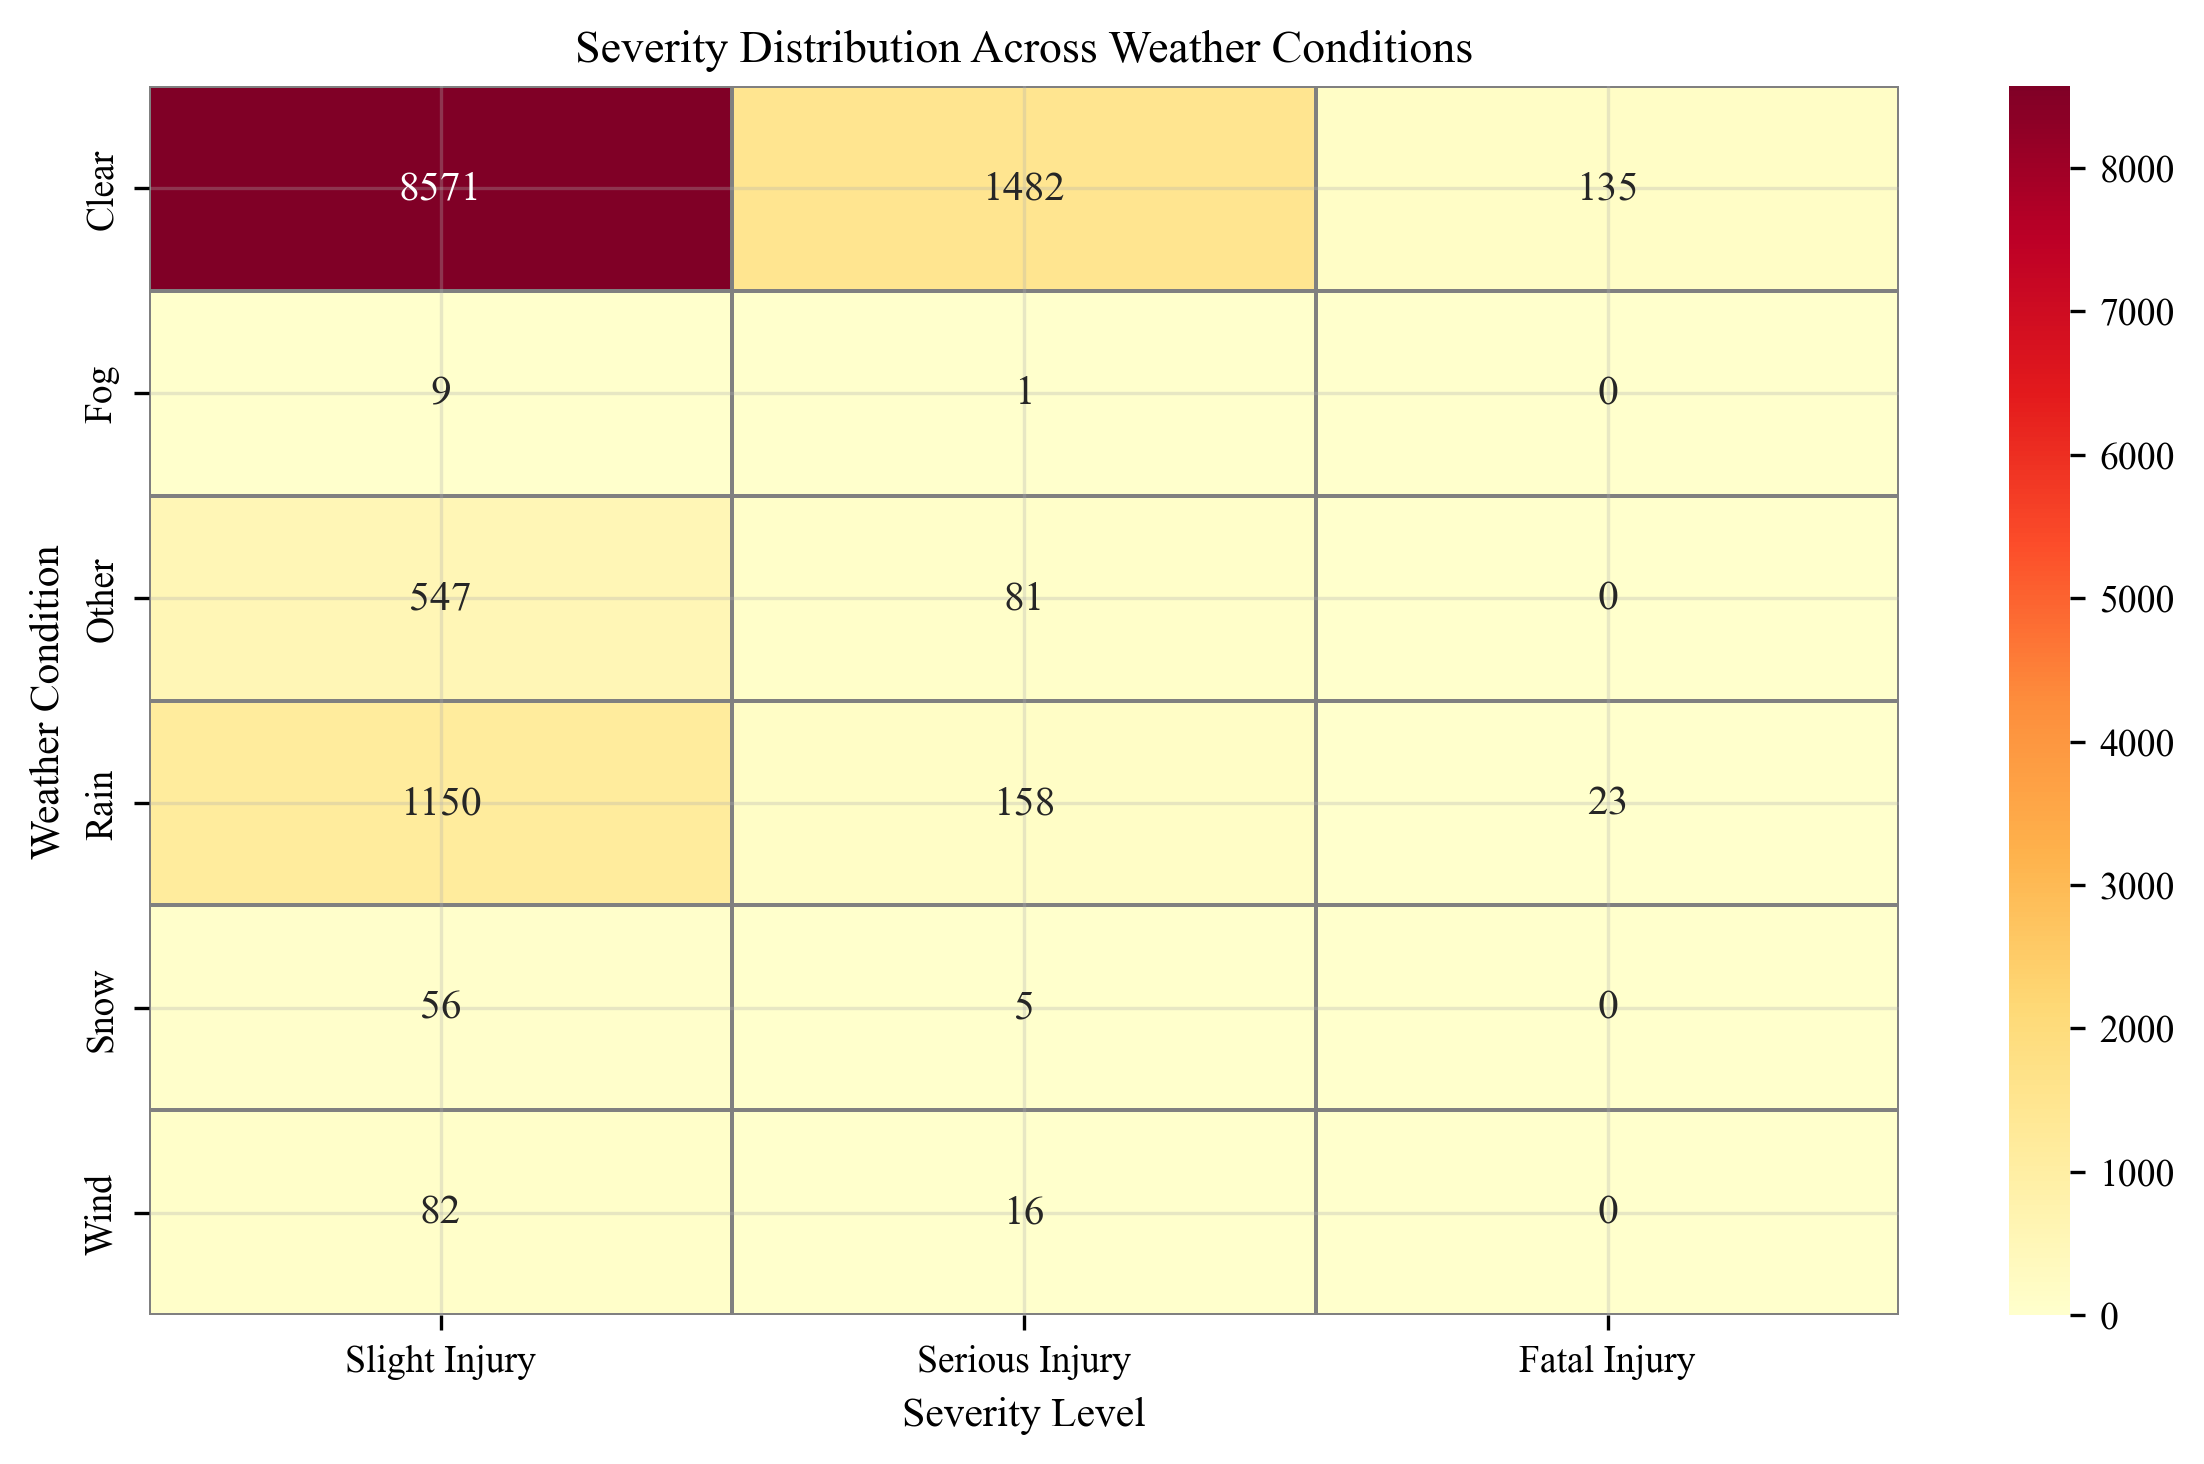
\includegraphics[width=\columnwidth]{figures/fig2_severity_weather_heatmap.png}}
\caption{Heatmap of severity distribution across weather conditions. Cell values show raw counts.}
\label{fig:weather_heatmap}
\end{figure}

\subsection{DBSCAN clustering results}

DBSCAN identified 9 clusters from the 12,316 geocoded records. No noise points were detected, largely because the chosen epsilon (287~km) is wide enough to capture dense metropolitan groupings.

Fig.~\ref{fig:dbscan} shows that the 9 clusters align broadly with major metropolitan regions, including Pune/Mumbai, Delhi NCR, Bangalore, Ahmedabad, Chennai, Kolkata, Nagpur, Varanasi, and Hyderabad.

\begin{figure}[htbp]
\centerline{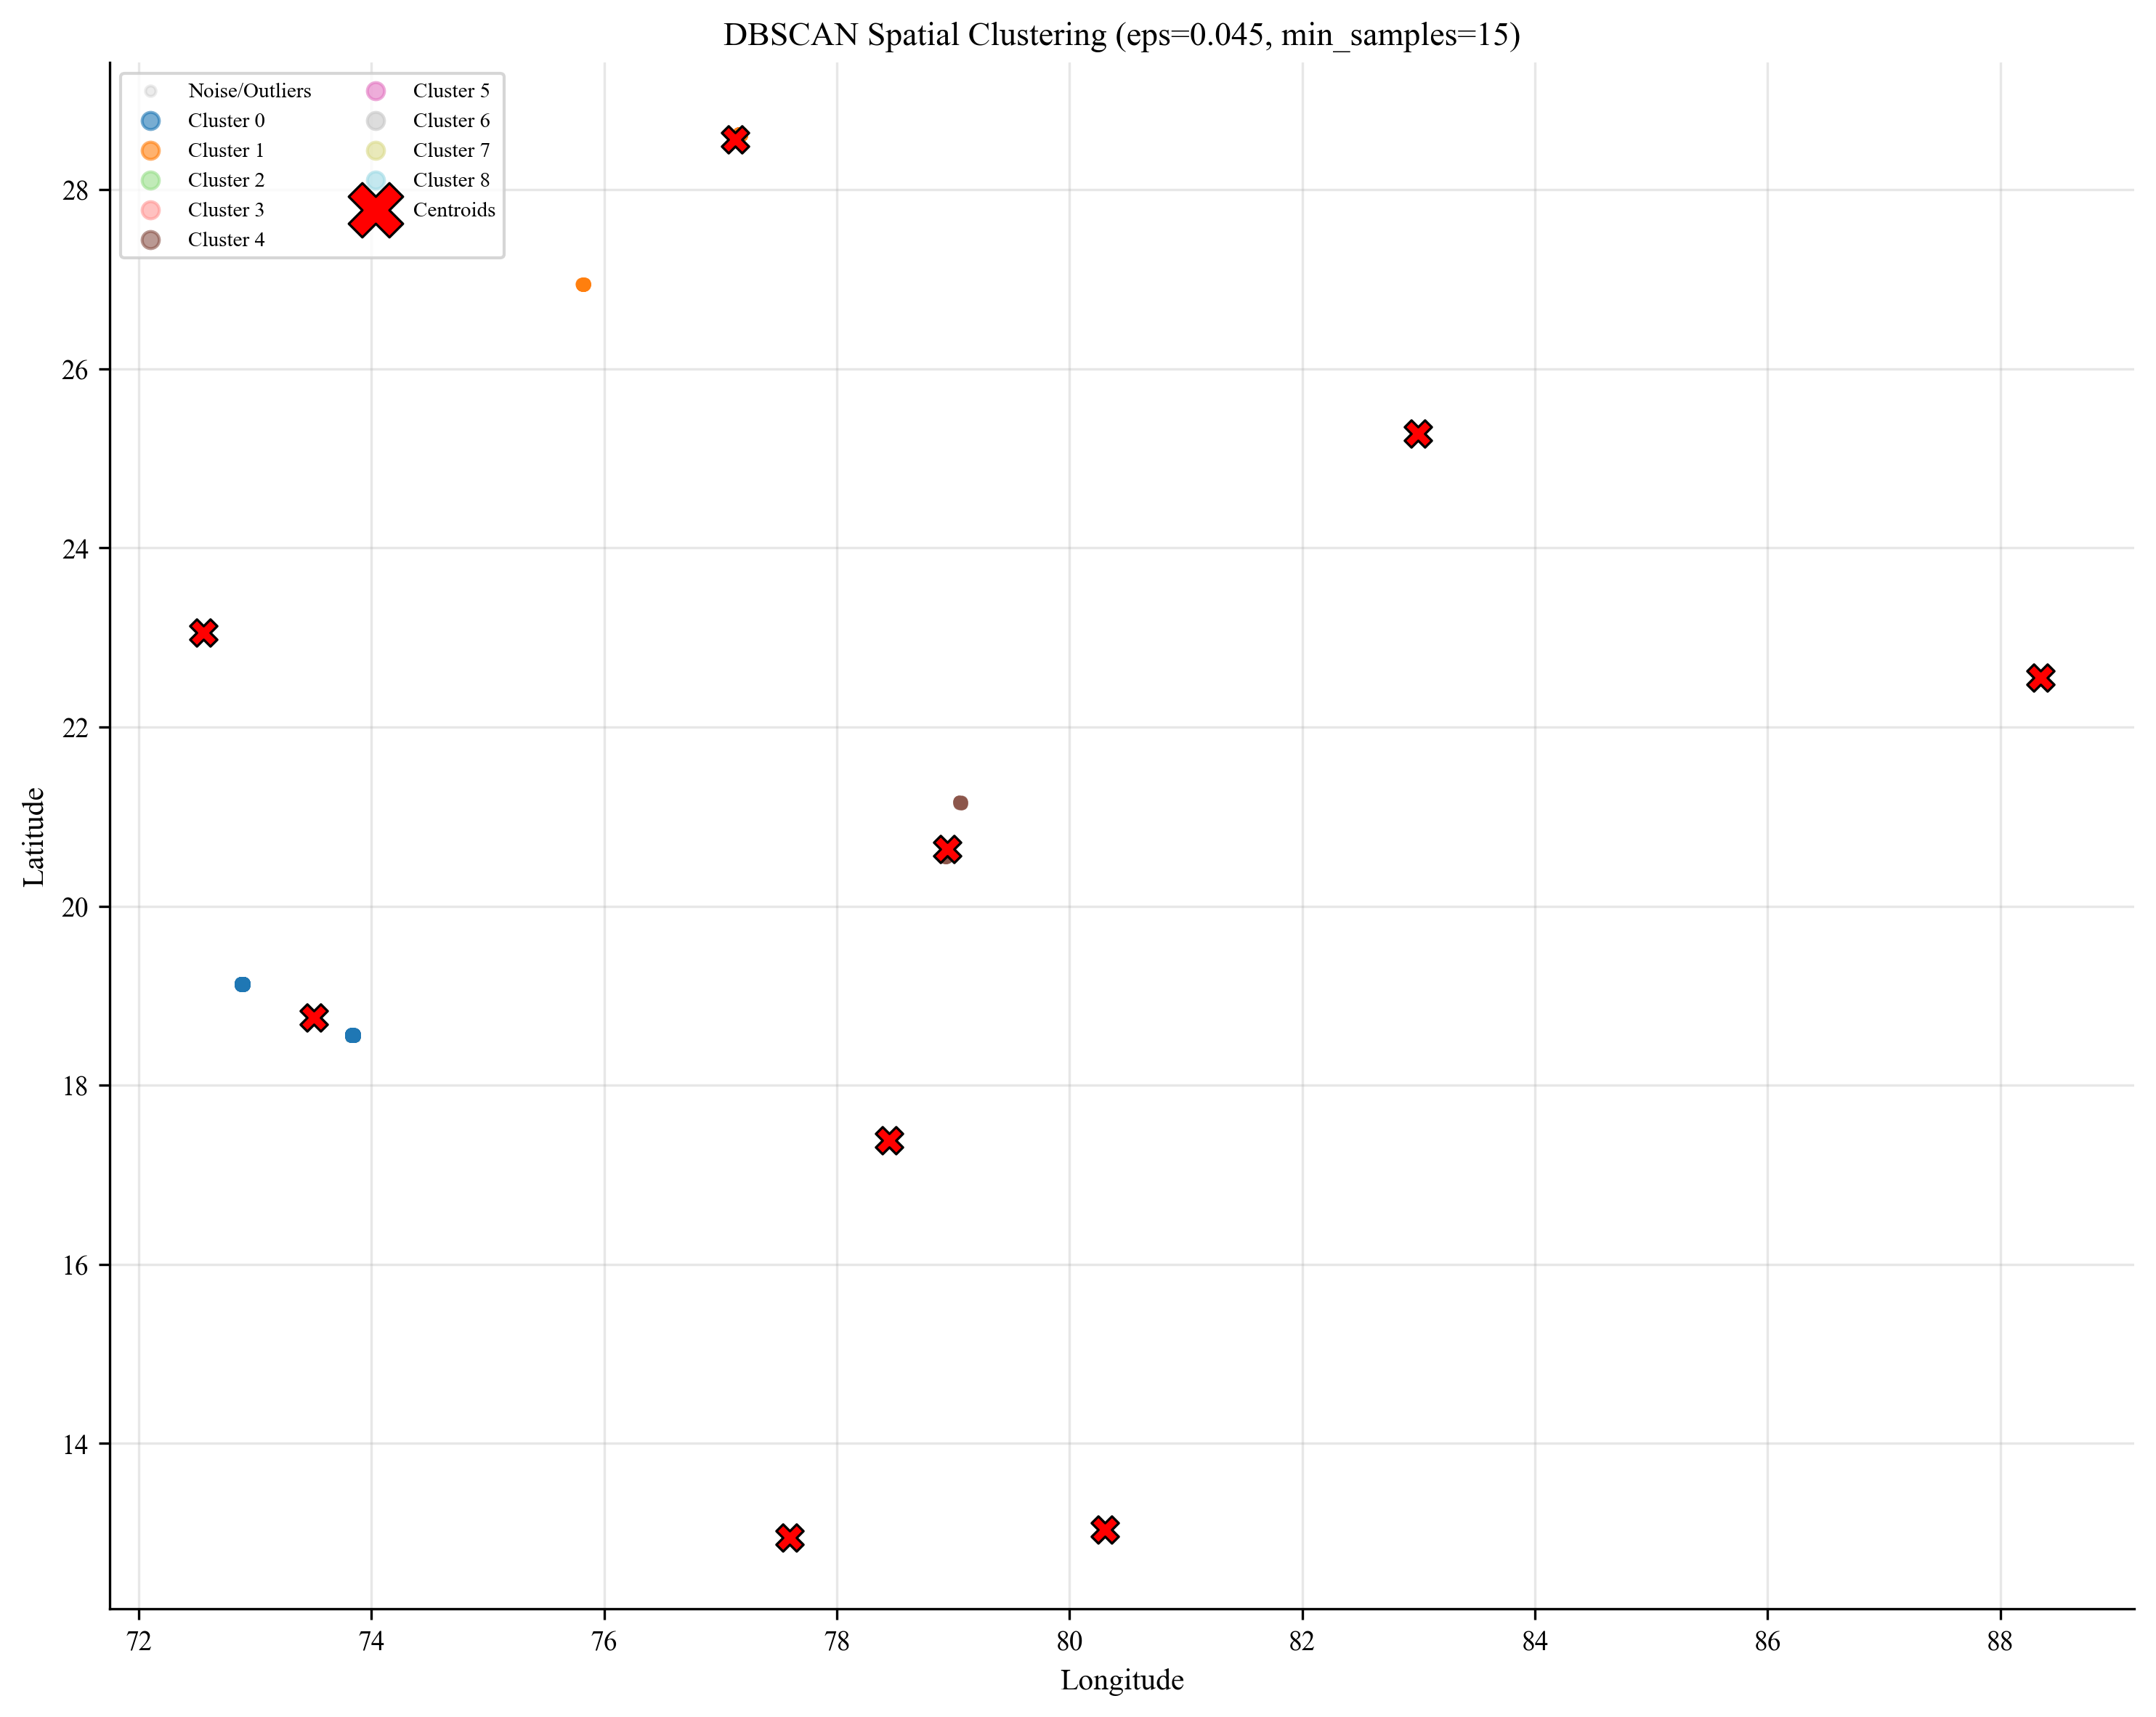
\includegraphics[width=\columnwidth]{figures/fig3_dbscan_clusters.png}}
\caption{Spatial distribution of 12,316 accident records, colored by DBSCAN cluster assignment. Red X markers indicate cluster centroids.}
\label{fig:dbscan}
\end{figure}

Table~\ref{tab:cluster_summary} shows that Cluster 0 (near Pune/Mumbai) is the largest, with 5,879 records, and that mean severity varies only slightly across clusters.

\begin{table}[htbp]
\caption{DBSCAN Cluster Summary}
\begin{center}
\footnotesize
\begin{tabular}{crrrrl}
\toprule
\textbf{ID} & \textbf{Lat} & \textbf{Lon} & \textbf{Count} & \textbf{Severity} & \textbf{Area} \\
\midrule
0 & 18.76 & 73.51 & 5,879 & 1.175 & Other \\
1 & 28.56 & 77.12 & 3,572 & 1.158 & Office \\
2 & 22.55 & 88.34 & 328 & 1.171 & Recreational \\
3 & 23.05 & 72.56 & 456 & 1.158 & Industrial \\
4 & 20.64 & 78.95 & 325 & 1.172 & Unknown \\
5 & 12.95 & 77.59 & 1,060 & 1.152 & Church \\
6 & 17.39 & 78.45 & 63 & 1.206 & Market \\
7 & 25.28 & 83.00 & 218 & 1.193 & Rural \\
8 & 13.04 & 80.30 & 415 & 1.154 & School \\
\bottomrule
\end{tabular}
\label{tab:cluster_summary}
\end{center}
\end{table}

\subsection{Classification performance}

The Random Forest classifier achieves 84.66\% test accuracy, but the per-class results in Table~\ref{tab:class_report} show that this performance is driven almost entirely by the Slight Injury class. Recall for Serious Injury falls to 1.43\%, and Fatal Injury is never predicted correctly.

\begin{table}[htbp]
\caption{Per-class Classification Report}
\begin{center}
\begin{tabular}{lcccc}
\toprule
\textbf{Class} & \textbf{Precision} & \textbf{Recall} & \textbf{F1} & \textbf{Support} \\
\midrule
Slight & 0.8473 & 0.9986 & 0.9167 & 2,084 \\
Serious & 0.6250 & 0.0143 & 0.0280 & 349 \\
Fatal & 0.0000 & 0.0000 & 0.0000 & 31 \\
\midrule
Macro avg & 0.4908 & 0.3376 & 0.3149 & 2,464 \\
Weighted avg & 0.8052 & 0.8466 & 0.7793 & 2,464 \\
\bottomrule
\end{tabular}
\label{tab:class_report}
\end{center}
\end{table}

This is a direct consequence of the 84:14:1 class ratio. Even with balanced class weights, the model still leans heavily toward the majority class. Fig.~\ref{fig:confusion} makes that visible: 344 of 349 Serious Injury samples and all 31 Fatal Injury samples are labeled as Slight.

\begin{figure}[htbp]
\centerline{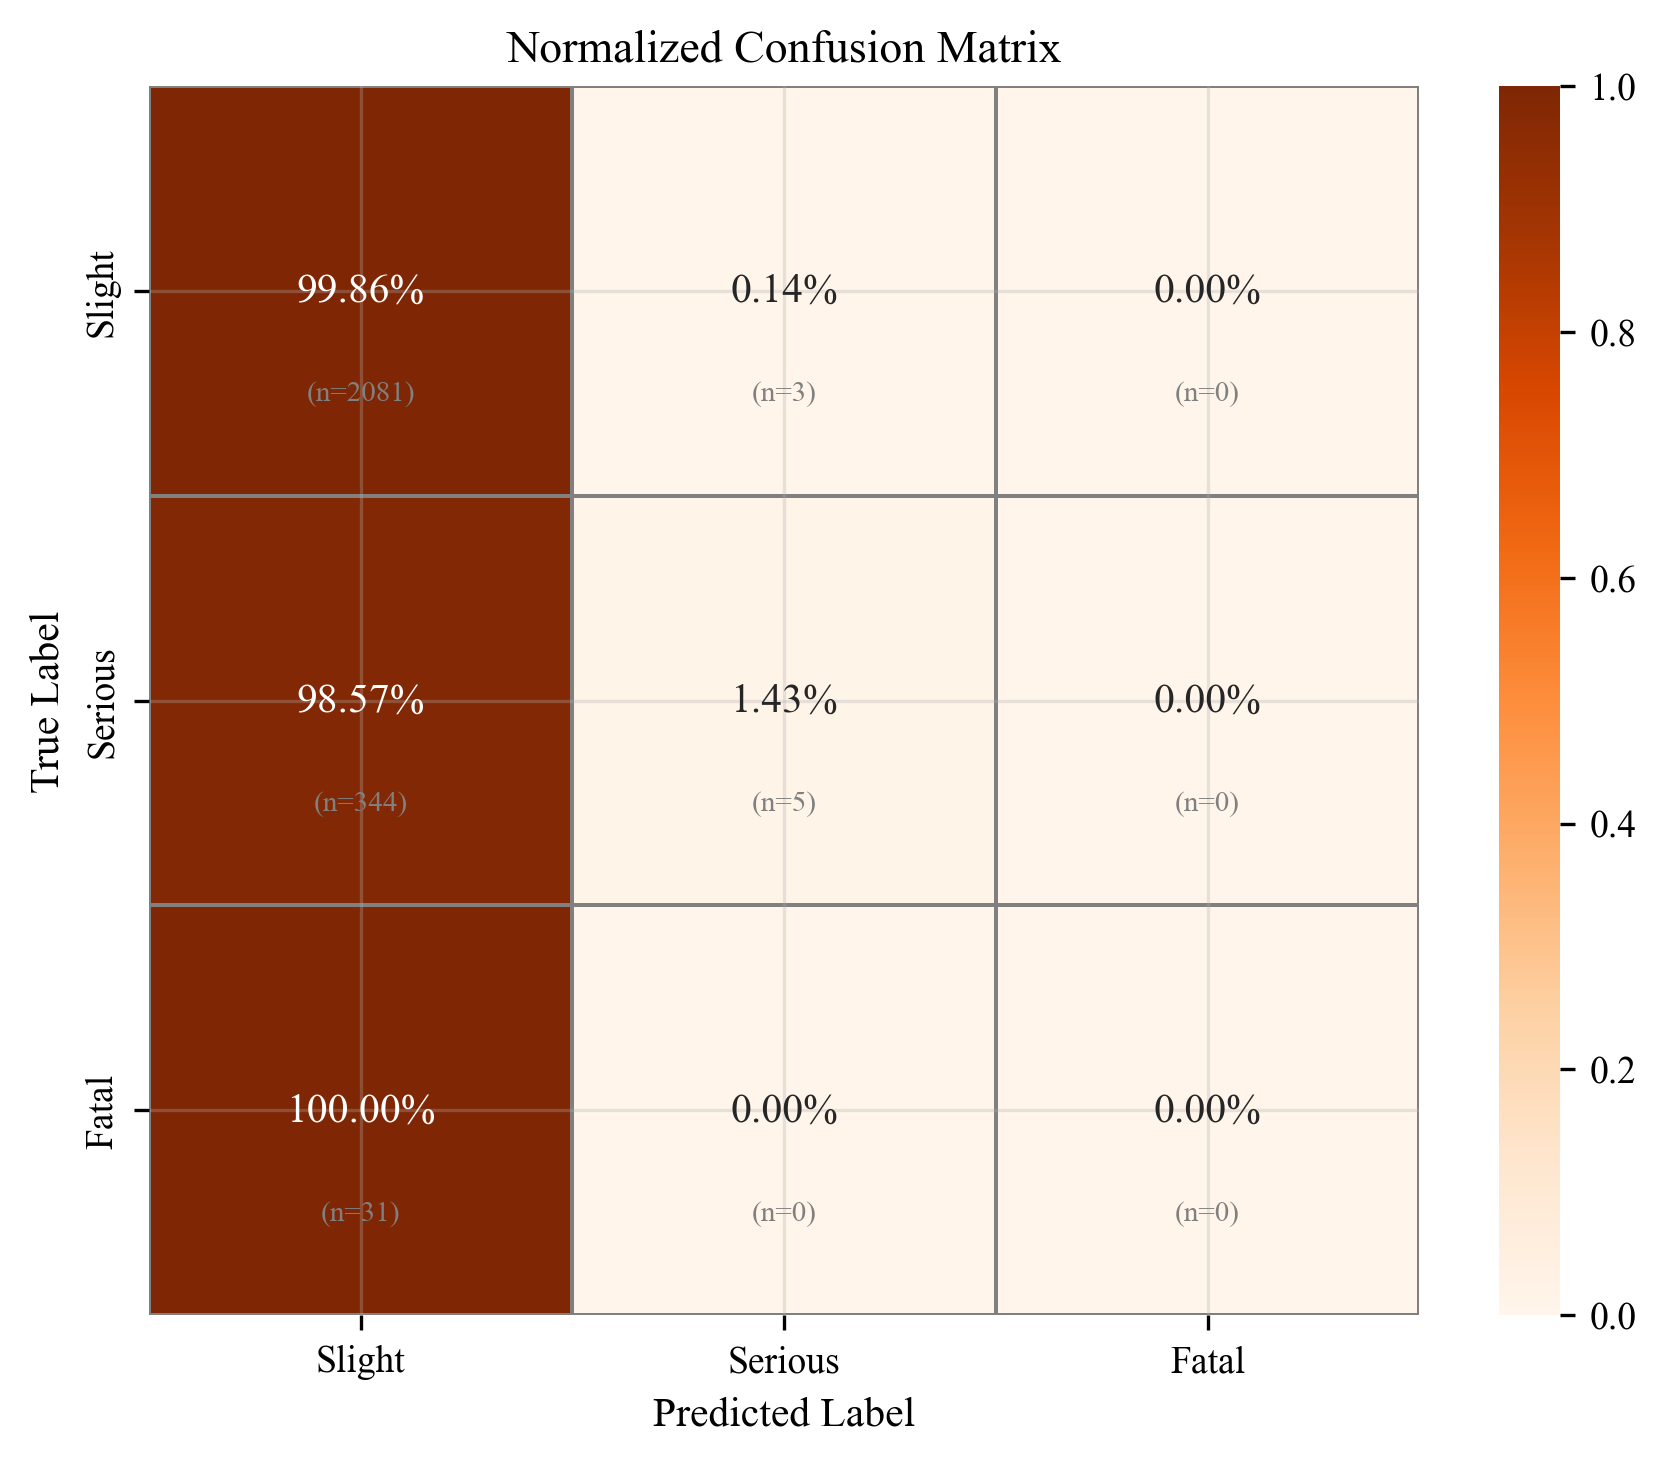
\includegraphics[width=0.85\columnwidth]{figures/fig4_confusion_matrix.png}}
\caption{Confusion matrix for the Random Forest classifier on the test set. The model predicts Slight Injury for nearly all inputs.}
\label{fig:confusion}
\end{figure}

The macro F1-score of 0.3149, Cohen's Kappa of 0.0198, and MCC of 0.0749 confirm that the model does not separate the minority classes well, even though the headline accuracy looks strong.

\textbf{ROC curves.} Fig.~\ref{fig:roc} shows one-vs-rest ROC curves with AUC values of 0.6918 for Slight, 0.6981 for Serious, and 0.8266 for Fatal. The relatively high Fatal AUC, despite zero recall, suggests that the model assigns somewhat higher fatal probabilities to those cases even though the final class decision never selects them.

\begin{figure}[htbp]
\centerline{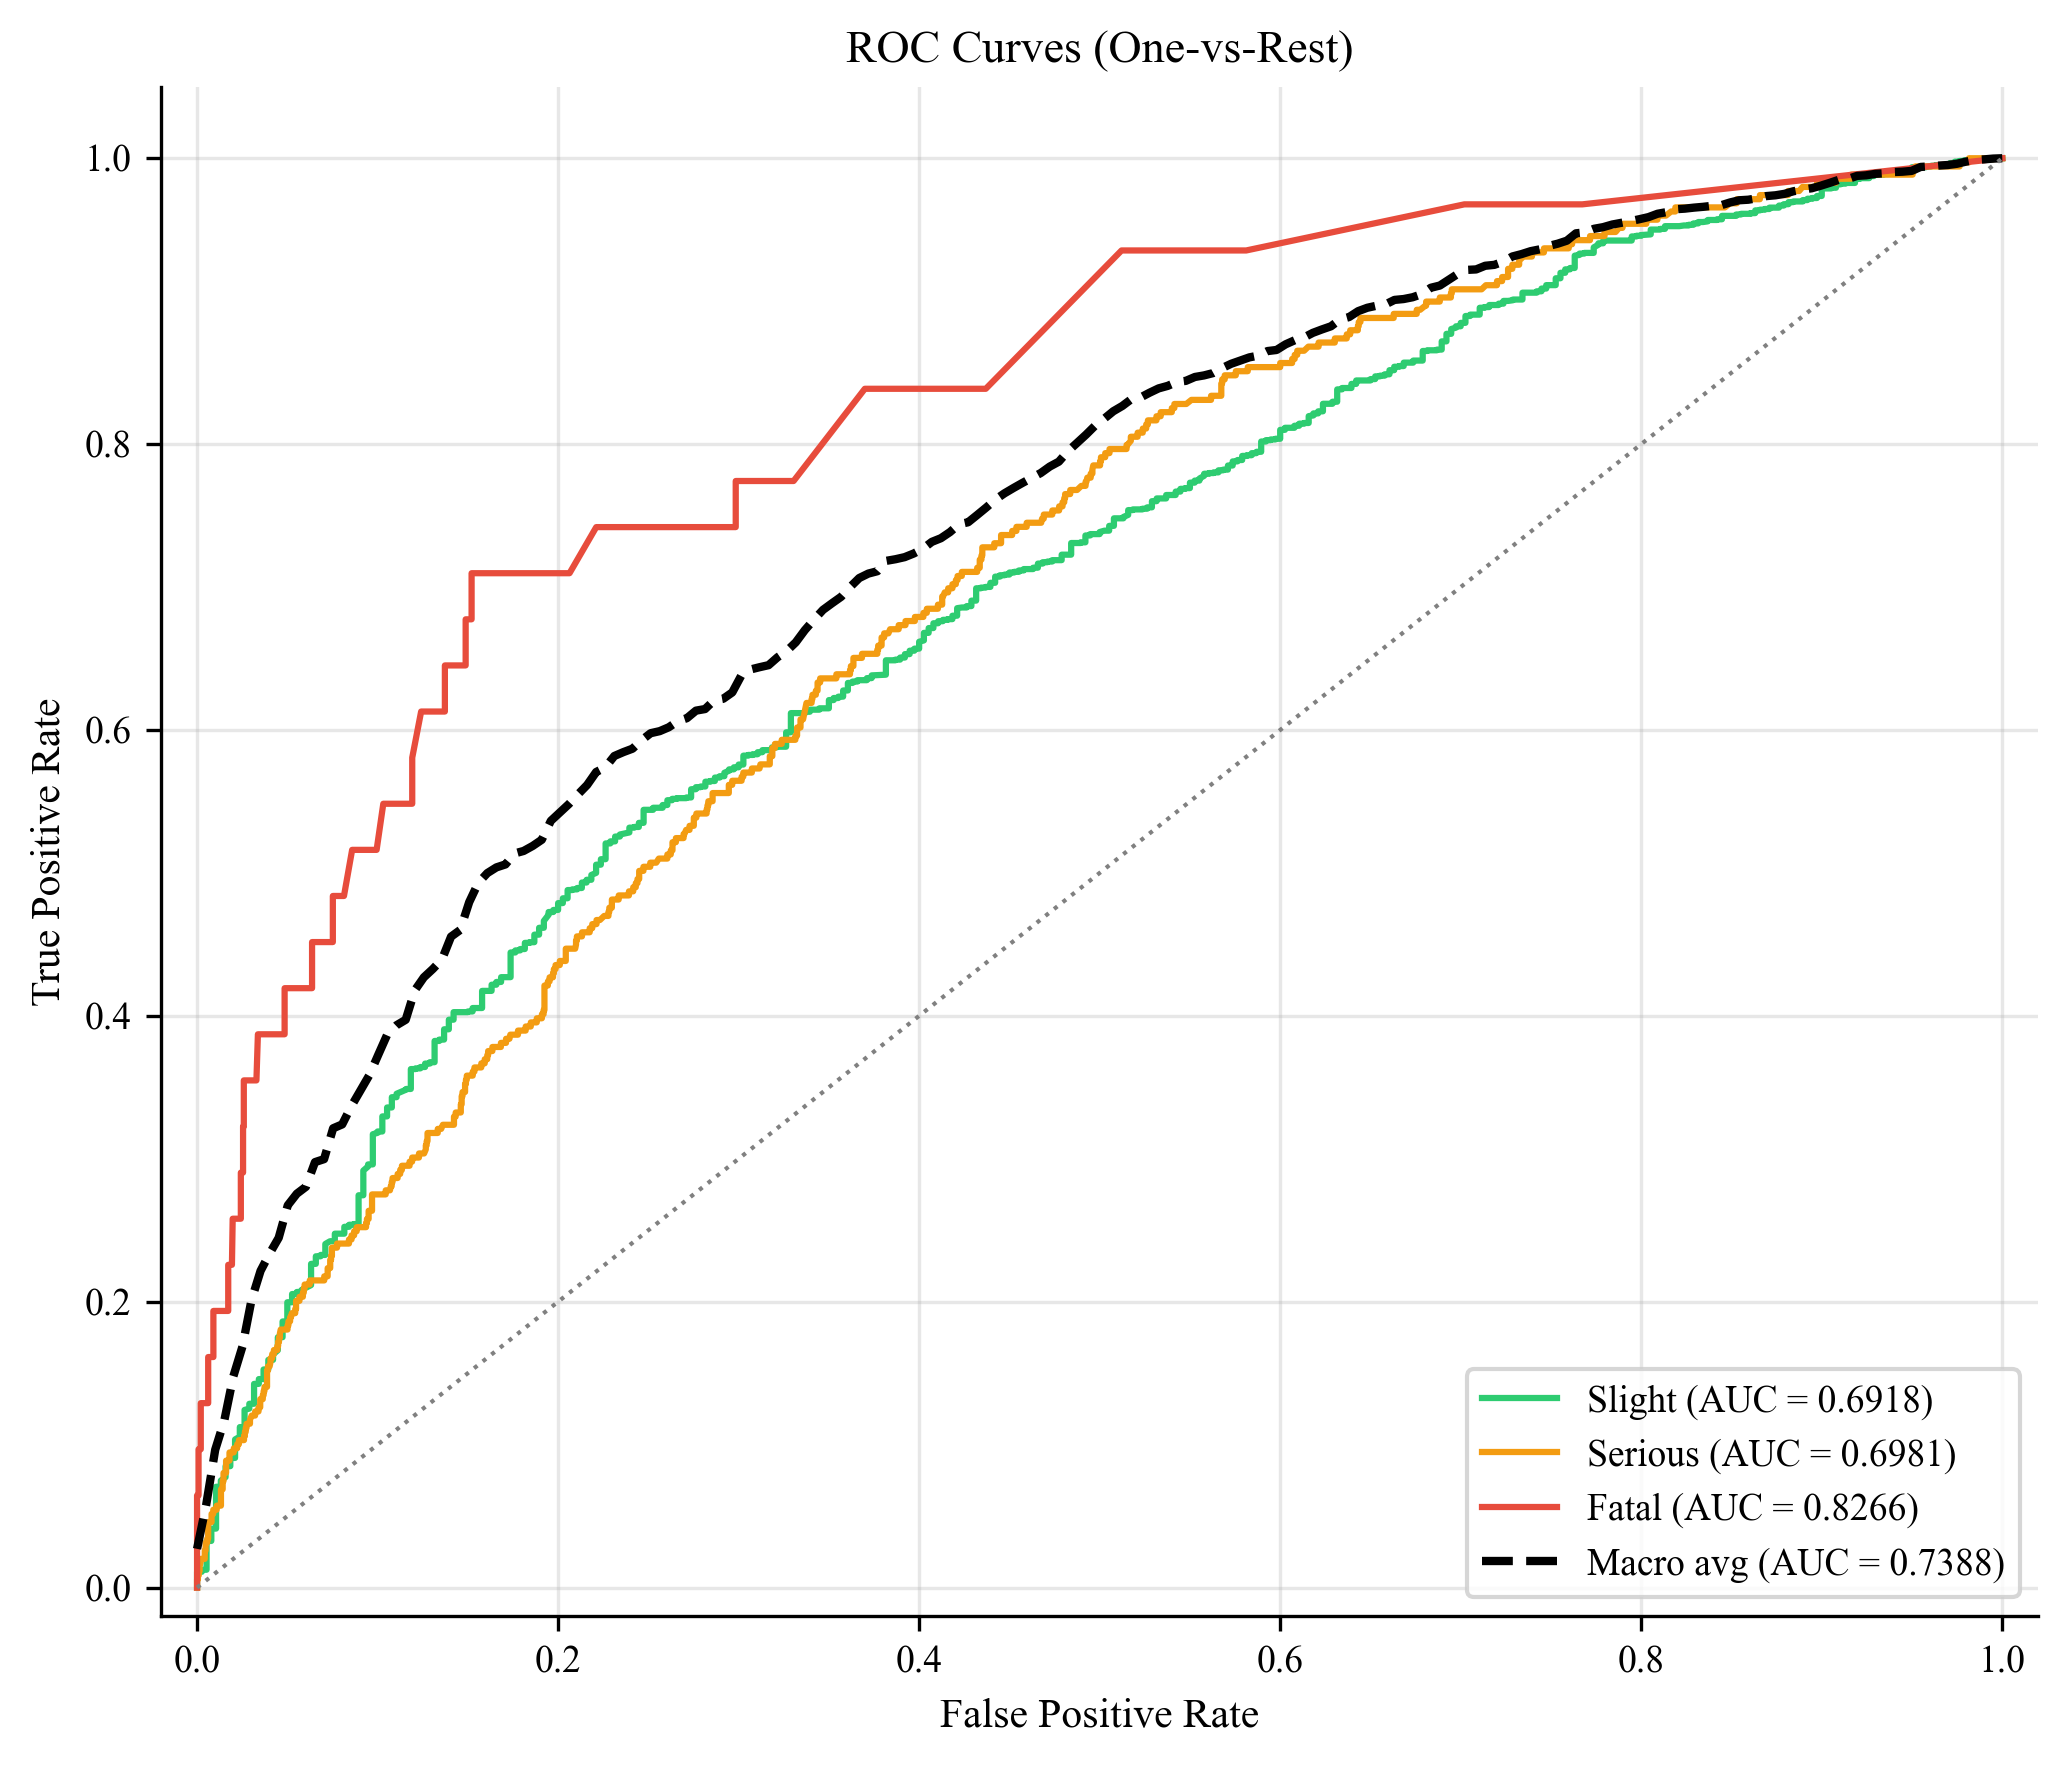
\includegraphics[width=\columnwidth]{figures/fig6_roc_curves.png}}
\caption{ROC curves (one-vs-rest) for three severity classes. Macro-average AUC = 0.7388.}
\label{fig:roc}
\end{figure}

\textbf{Feature importances.} Fig.~\ref{fig:feat_imp} shows that hour of day, cause of accident, and day of week are the three strongest predictors. Cluster\_ID ranks ninth with an importance of 0.0607, which shows that spatial context contributes useful information.

\begin{figure}[htbp]
\centerline{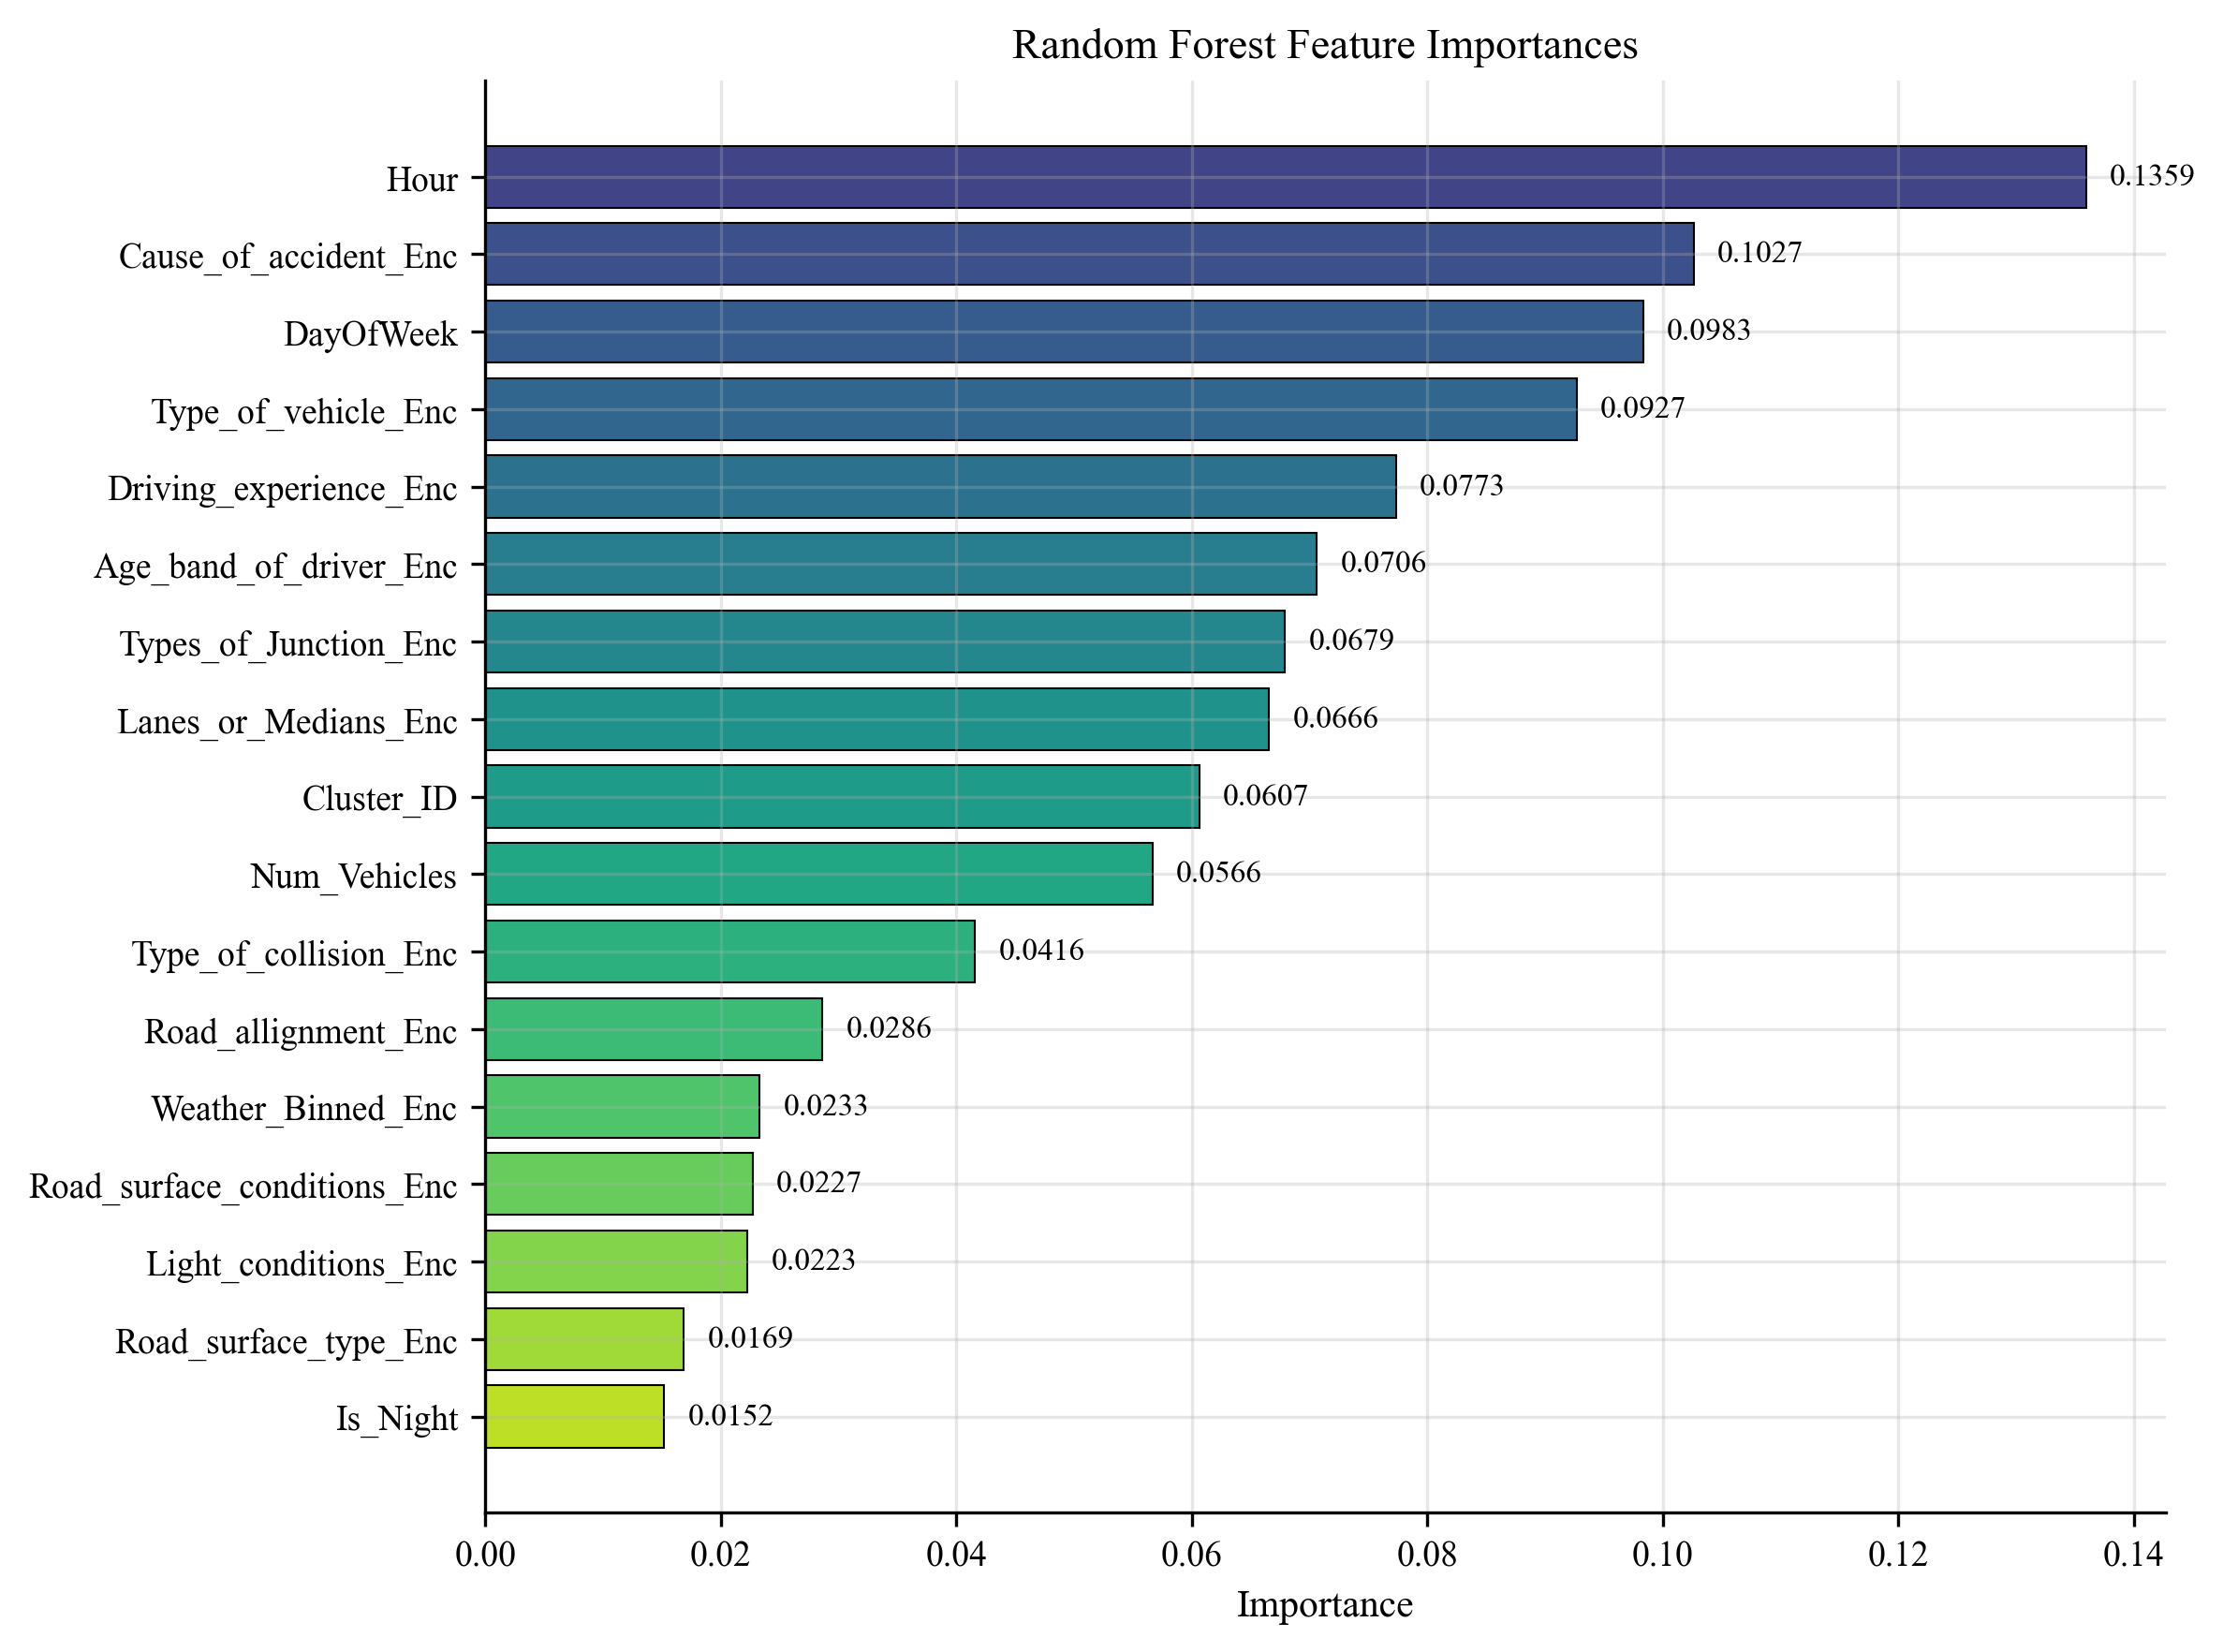
\includegraphics[width=\columnwidth]{figures/fig5_feature_importances.png}}
\caption{Random Forest feature importances ranked by contribution. Hour of day is the strongest predictor.}
\label{fig:feat_imp}
\end{figure}

Table~\ref{tab:top_features} lists the top 10 features with their importance scores.

\begin{table}[htbp]
\caption{Top 10 Feature Importances}
\begin{center}
\begin{tabular}{clc}
\toprule
\textbf{Rank} & \textbf{Feature} & \textbf{Importance} \\
\midrule
1 & Hour & 0.1359 \\
2 & Cause\_of\_accident & 0.1027 \\
3 & DayOfWeek & 0.0983 \\
4 & Type\_of\_vehicle & 0.0927 \\
5 & Driving\_experience & 0.0773 \\
6 & Age\_band\_of\_driver & 0.0706 \\
7 & Types\_of\_Junction & 0.0679 \\
8 & Lanes\_or\_Medians & 0.0666 \\
9 & Cluster\_ID & 0.0607 \\
10 & Num\_Vehicles & 0.0566 \\
\bottomrule
\end{tabular}
\label{tab:top_features}
\end{center}
\end{table}

Environmental features rank in the lower part of the importance list, suggesting that weather and road-condition variation in this dataset adds less predictive separation than temporal, vehicle, and driver-related variables.

\textbf{Learning curve.} Fig.~\ref{fig:learning} shows clear overfitting: training accuracy reaches 1.0 while validation accuracy plateaus near 0.85.

\begin{figure}[htbp]
\centerline{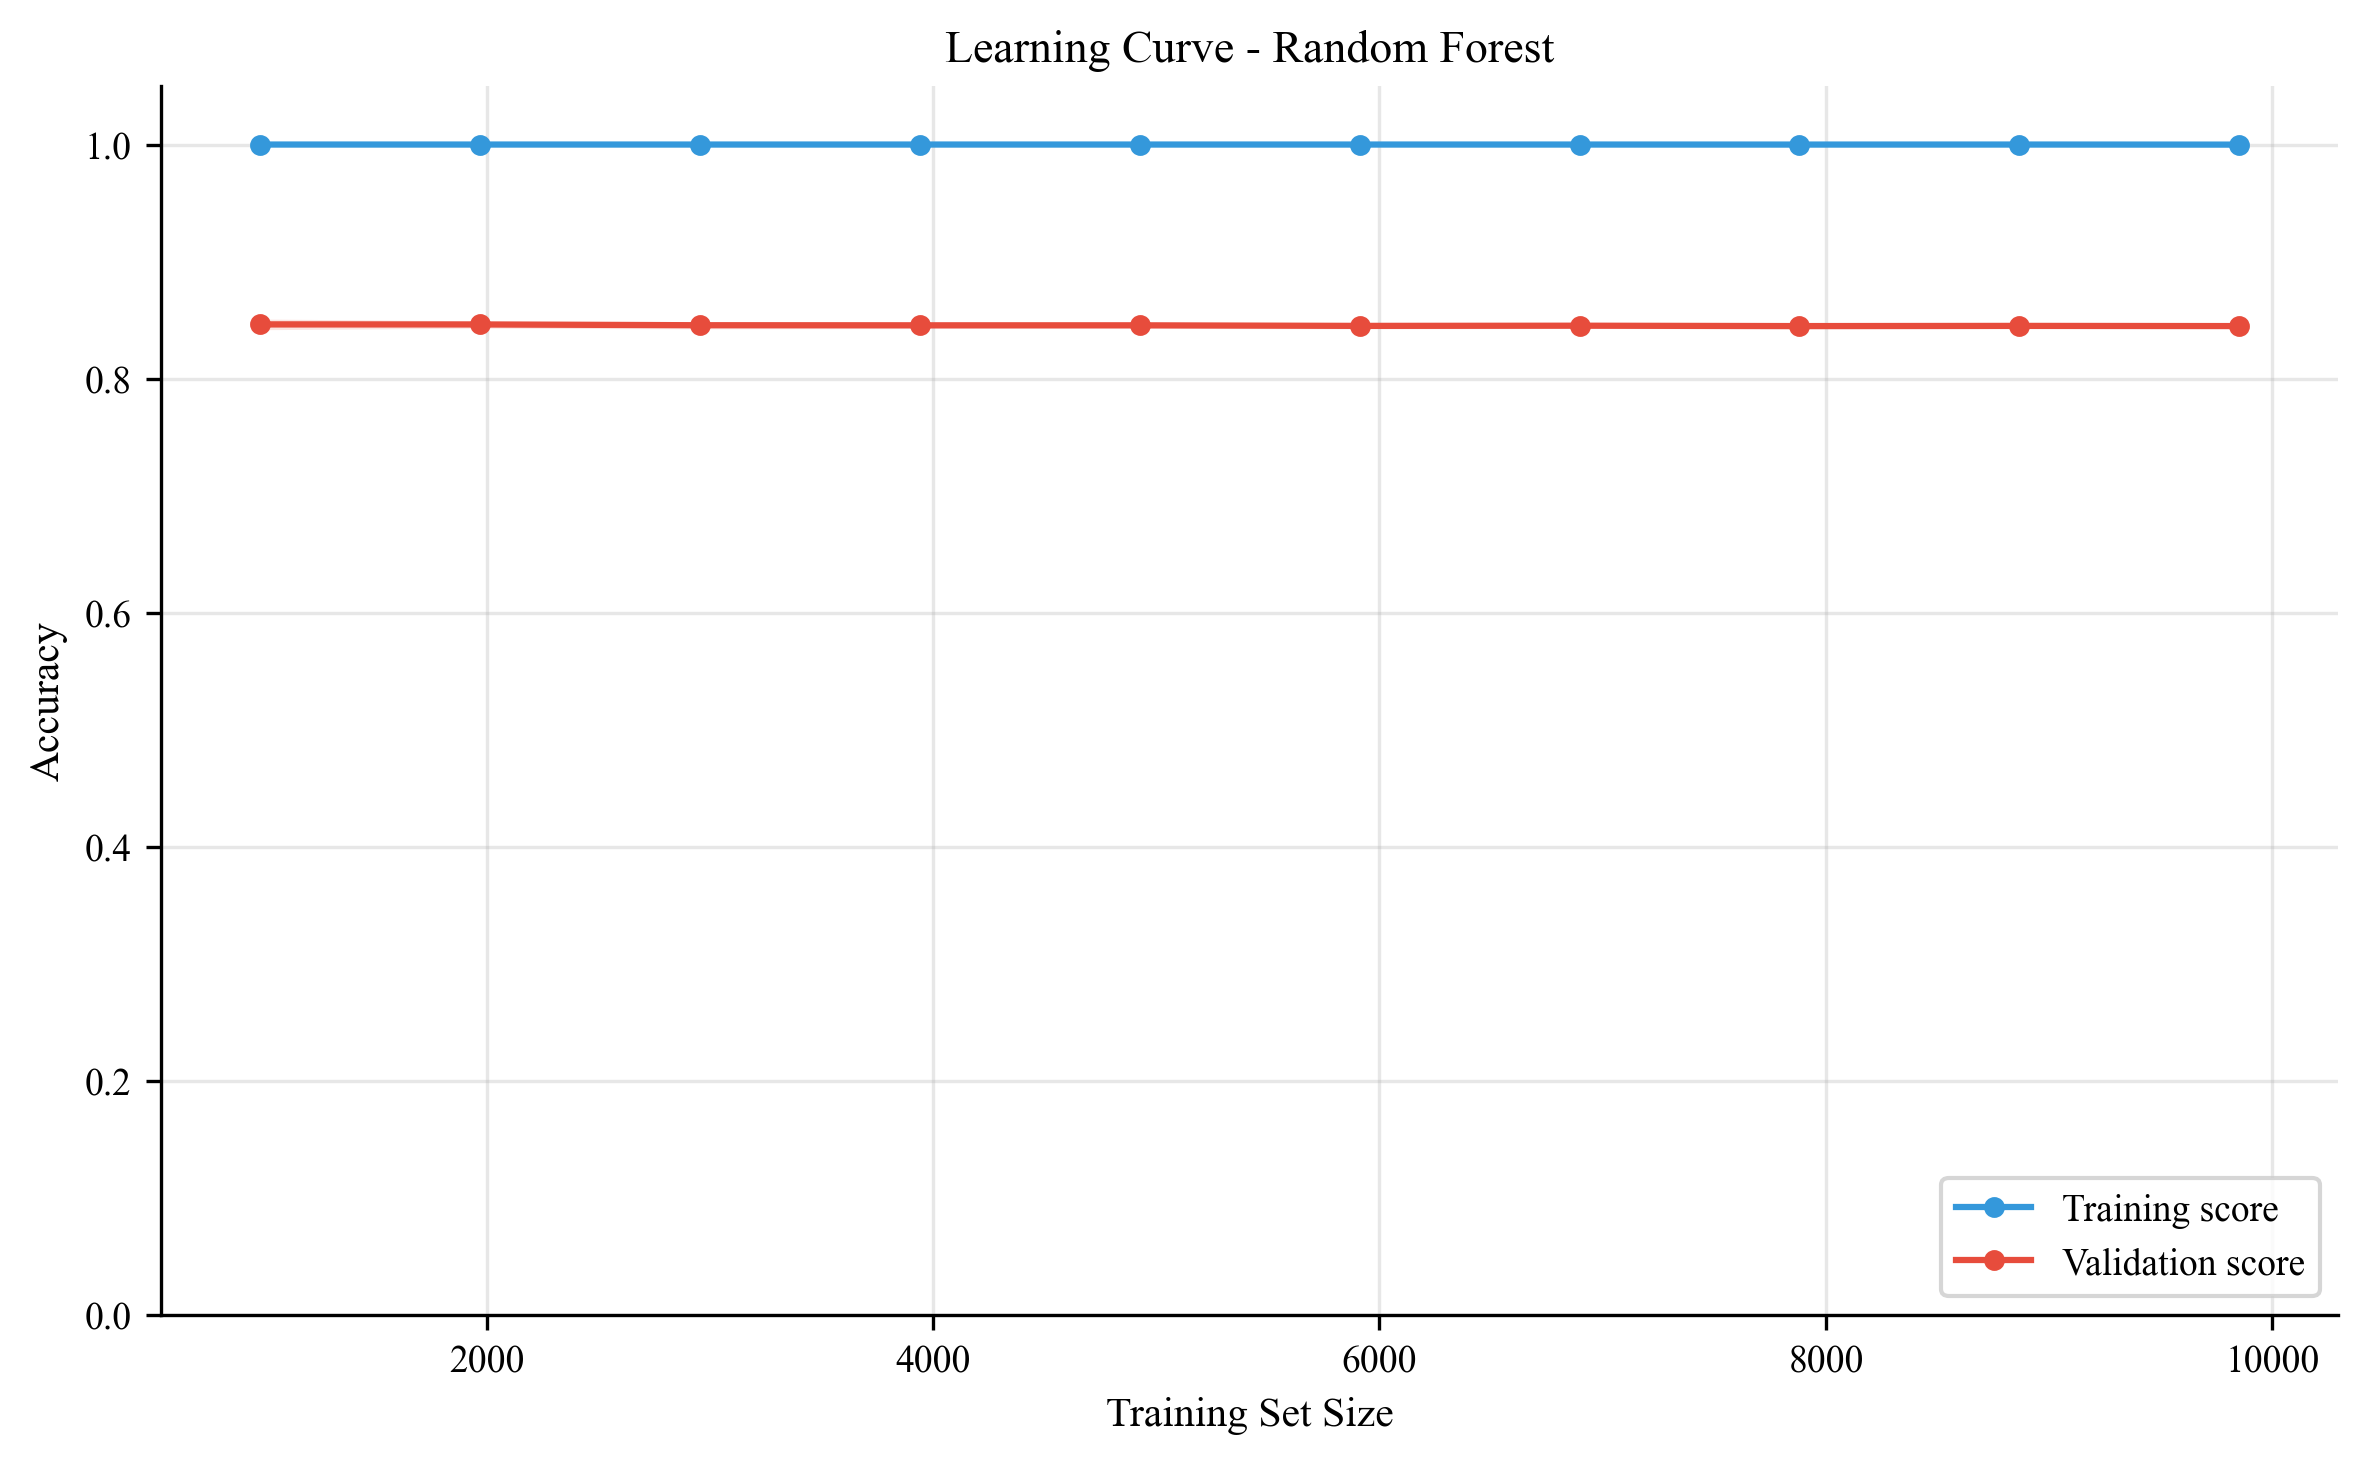
\includegraphics[width=\columnwidth]{figures/fig7_learning_curve.png}}
\caption{Learning curve for the Random Forest classifier. The persistent gap between training and validation scores indicates overfitting.}
\label{fig:learning}
\end{figure}

\textbf{Cross-validation.} Table~\ref{tab:cv_results} shows stable accuracy across five folds ($0.8476 \pm 0.0010$), while macro F1 varies more ($0.3251 \pm 0.0112$), reflecting unstable minority-class predictions.

\begin{table}[htbp]
\caption{Five-fold Stratified Cross-validation Results}
\begin{center}
\footnotesize
\begin{tabular}{ccccc}
\toprule
\textbf{Fold} & \textbf{Accuracy} & \textbf{F1 (macro)} & \textbf{Precision} & \textbf{Recall} \\
\midrule
1 & 0.8466 & 0.3150 & 0.4908 & 0.3378 \\
2 & 0.8486 & 0.3208 & 0.5791 & 0.3408 \\
3 & 0.8490 & 0.3417 & 0.9125 & 0.3516 \\
4 & 0.8473 & 0.3133 & 0.6157 & 0.3372 \\
5 & 0.8465 & 0.3345 & 0.6575 & 0.3479 \\
\midrule
Mean & 0.8476 & 0.3251 & 0.6511 & 0.3430 \\
Std & 0.0010 & 0.0112 & 0.1418 & 0.0057 \\
\bottomrule
\end{tabular}
\label{tab:cv_results}
\end{center}
\end{table}

\subsection{Comparative analysis}

To place the Random Forest results in context, five additional classifiers were trained on the same split and feature set. Table~\ref{tab:model_comparison} shows that Random Forest has the highest accuracy, while Decision Tree attains the highest macro F1-score by making slightly more balanced predictions.

\begin{table}[htbp]
\caption{Comparative Performance of Classification Models}
\begin{center}
\footnotesize
\begin{tabular}{lccccc}
\toprule
\textbf{Model} & \textbf{Acc.} & \textbf{Prec.} & \textbf{Rec.} & \textbf{F1} & \textbf{$\kappa$} \\
\midrule
Decision Tree & 0.737 & 0.352 & 0.353 & 0.352 & 0.068 \\
Random Forest & 0.847 & 0.491 & 0.338 & 0.315 & 0.020 \\
Naive Bayes & 0.843 & 0.359 & 0.335 & 0.310 & 0.006 \\
KNN & 0.839 & 0.312 & 0.332 & 0.308 & -0.006 \\
SVM (RBF) & 0.500 & 0.355 & 0.408 & 0.306 & 0.046 \\
Logistic Reg. & 0.436 & 0.360 & 0.446 & 0.291 & 0.043 \\
\bottomrule
\end{tabular}
\label{tab:model_comparison}
\end{center}
\end{table}

All models show low Cohen's Kappa values, which means minority-class separation remains weak. The available features capture temporal and spatial patterns better than crash dynamics.

\subsection{Accident Risk Index results}

The ARI was computed for all 9 clusters using the formula in (\ref{eq:ari}) with derived weights $W_1 = 0.534$, $W_2 = 0.401$, $W_3 = 0.065$. Table~\ref{tab:ari_results} shows the component scores and final ARI for each cluster.

\begin{table}[htbp]
\caption{Accident Risk Index Results per Cluster}
\begin{center}
\footnotesize
\begin{tabular}{cccccl}
\toprule
\textbf{ID} & $S_{sev}$ & $S_{dens}$ & $S_{env}$ & \textbf{ARI} & \textbf{Tier} \\
\midrule
0 & 0.428 & 1.000 & 0.15 & 0.639 & Severe \\
1 & 0.116 & 0.608 & 0.15 & 0.315 & Moderate \\
6 & 1.000 & 0.011 & 0.15 & 0.548 & Severe \\
7 & 0.749 & 0.037 & 0.15 & 0.424 & Moderate \\
4 & 0.375 & 0.055 & 0.15 & 0.232 & Low \\
2 & 0.346 & 0.056 & 0.15 & 0.217 & Low \\
3 & 0.110 & 0.078 & 0.15 & 0.100 & Low \\
5 & 0.000 & 0.180 & 0.15 & 0.082 & Low \\
8 & 0.043 & 0.071 & 0.15 & 0.061 & Low \\
\bottomrule
\end{tabular}
\label{tab:ari_results}
\end{center}
\end{table}

ARI scores range from 0.061 (Cluster 8, Chennai area) to 0.639 (Cluster 0, Pune/Mumbai area). No cluster reaches the Critical tier. Cluster 0 ranks highest because it combines the greatest density with moderate severity, while Cluster 6 reaches the Severe tier mainly because of its high severity score despite a small incident count.

Fig.~\ref{fig:risk_map} shows the risk map, where each cluster centroid is plotted with a color corresponding to its ARI score and a bubble size proportional to incident count.

\begin{figure}[htbp]
\centerline{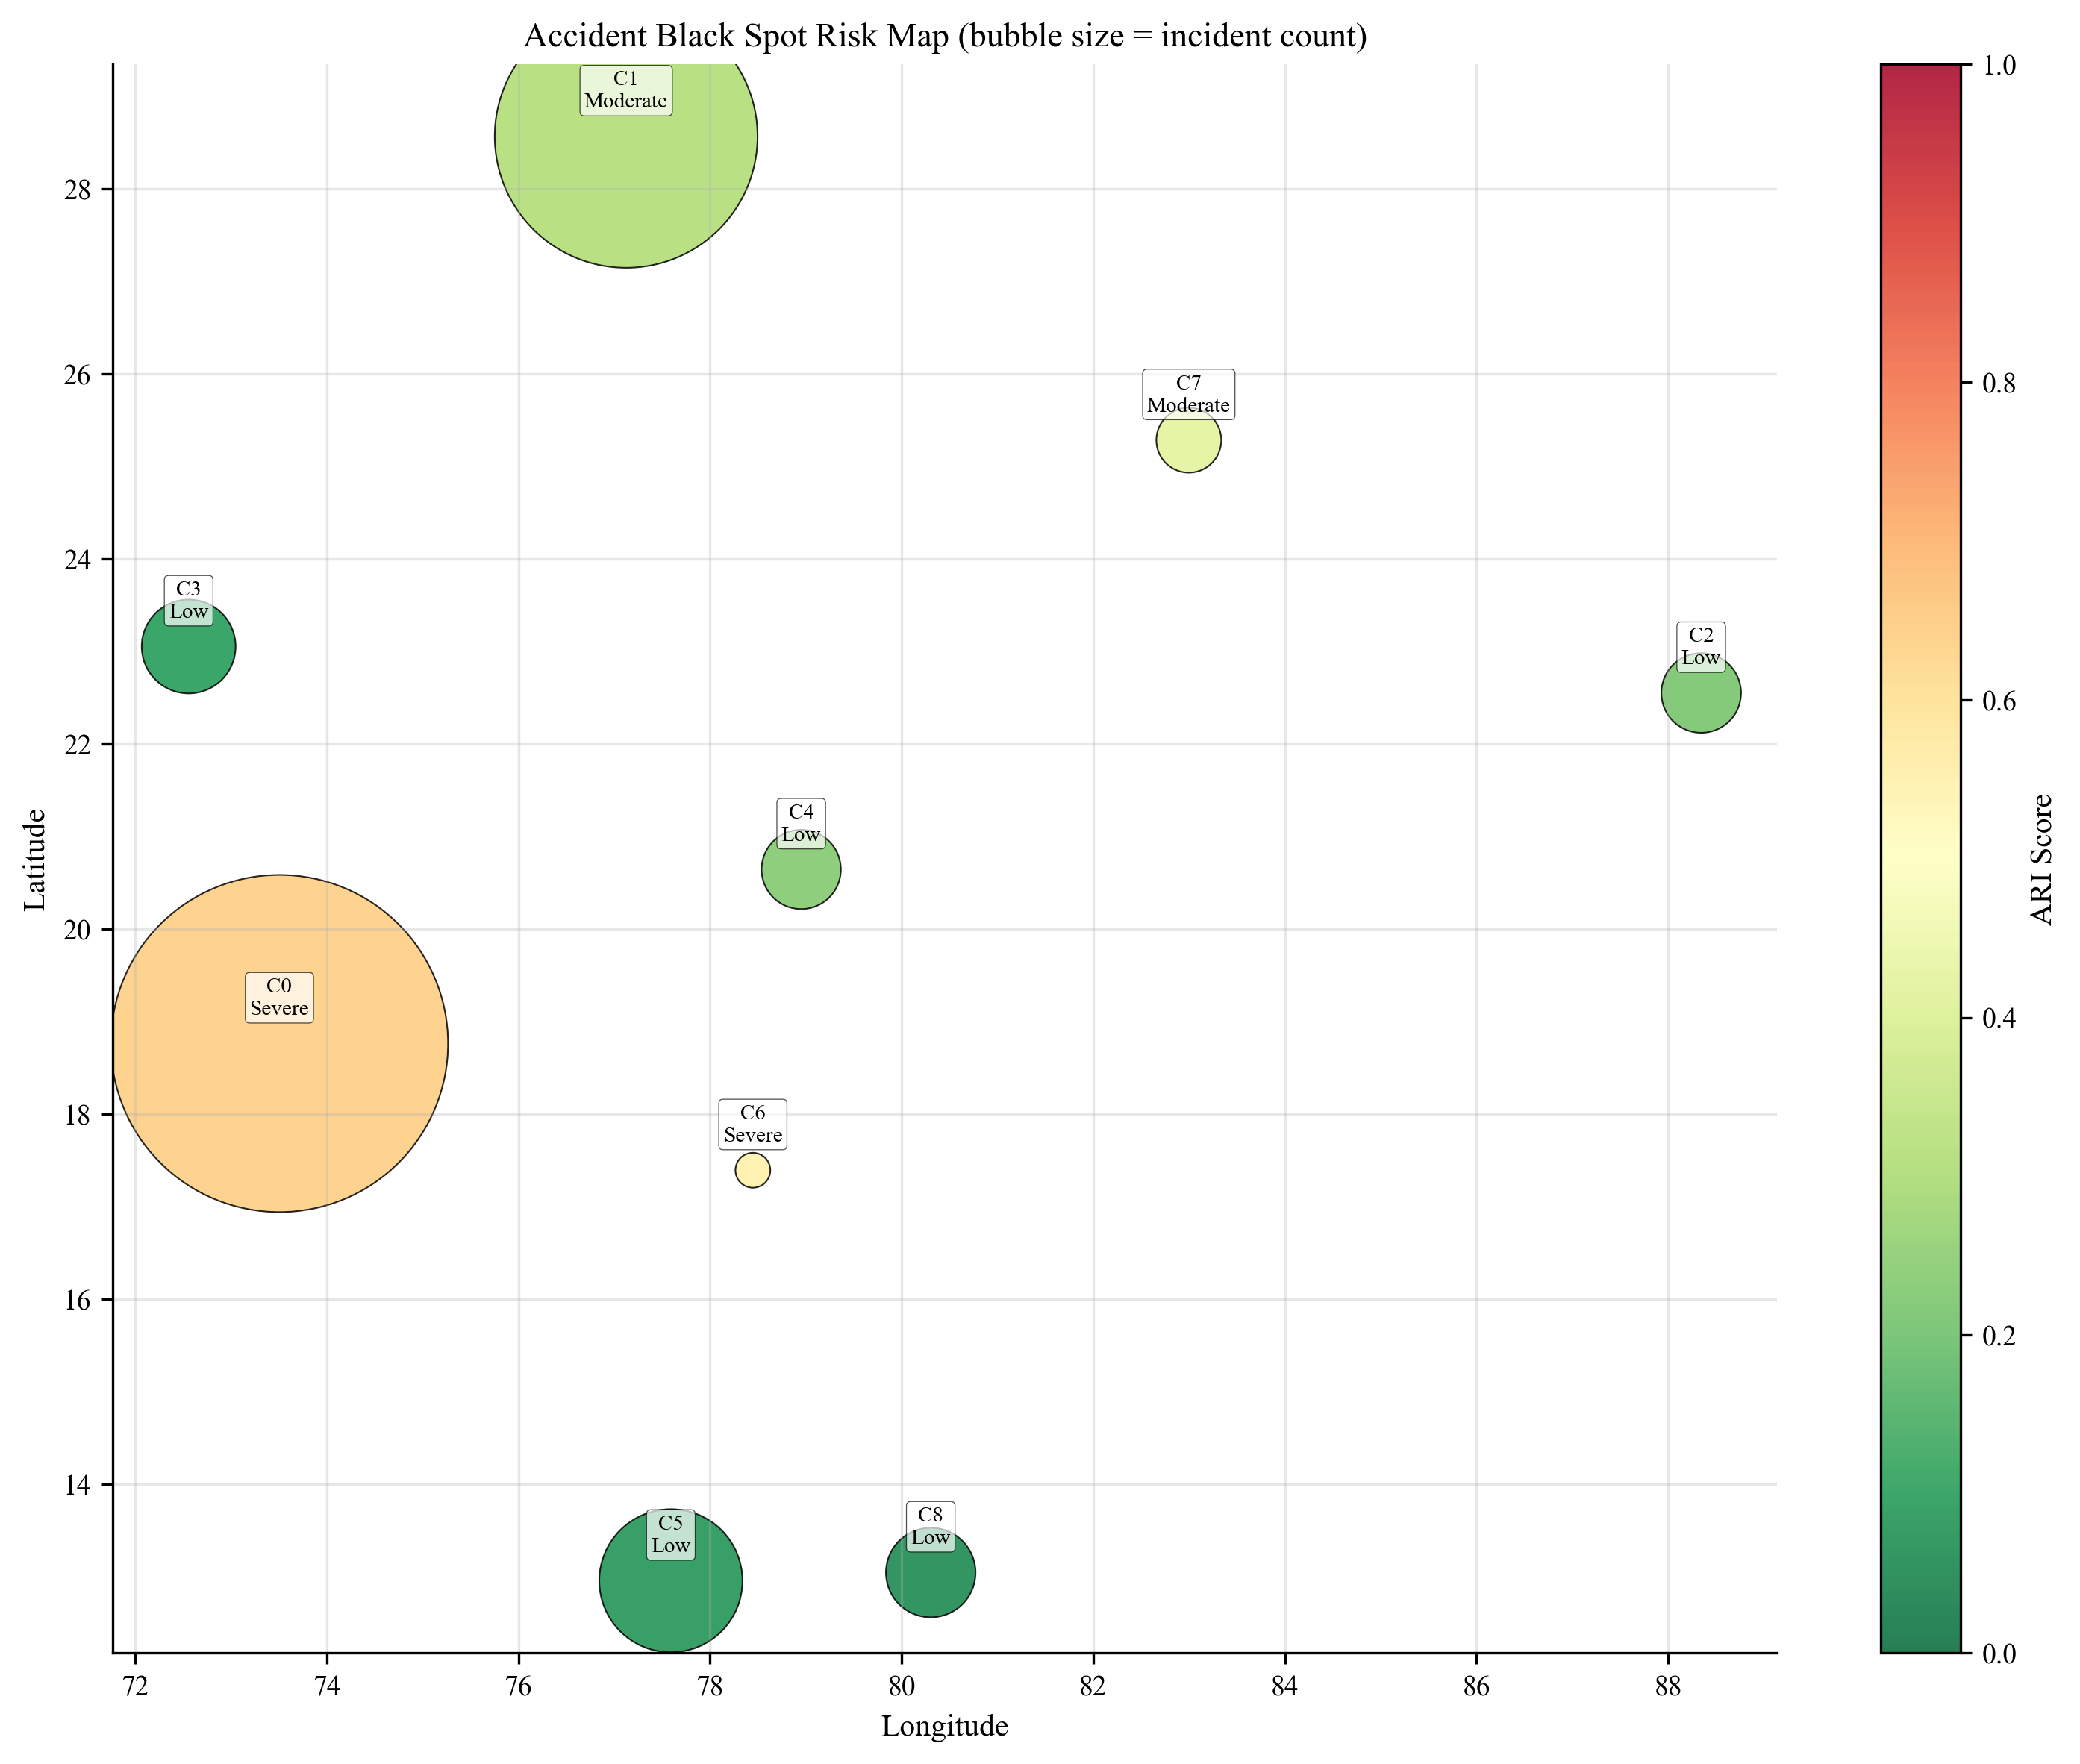
\includegraphics[width=\columnwidth]{figures/fig8_risk_map.png}}
\caption{Accident black spot risk map. Circle size is proportional to incident count; color indicates ARI score (green = low, red = high).}
\label{fig:risk_map}
\end{figure}

Fig.~\ref{fig:cluster_sev} shows the severity composition across clusters, illustrating how severity varies geographically.

\begin{figure}[htbp]
\centerline{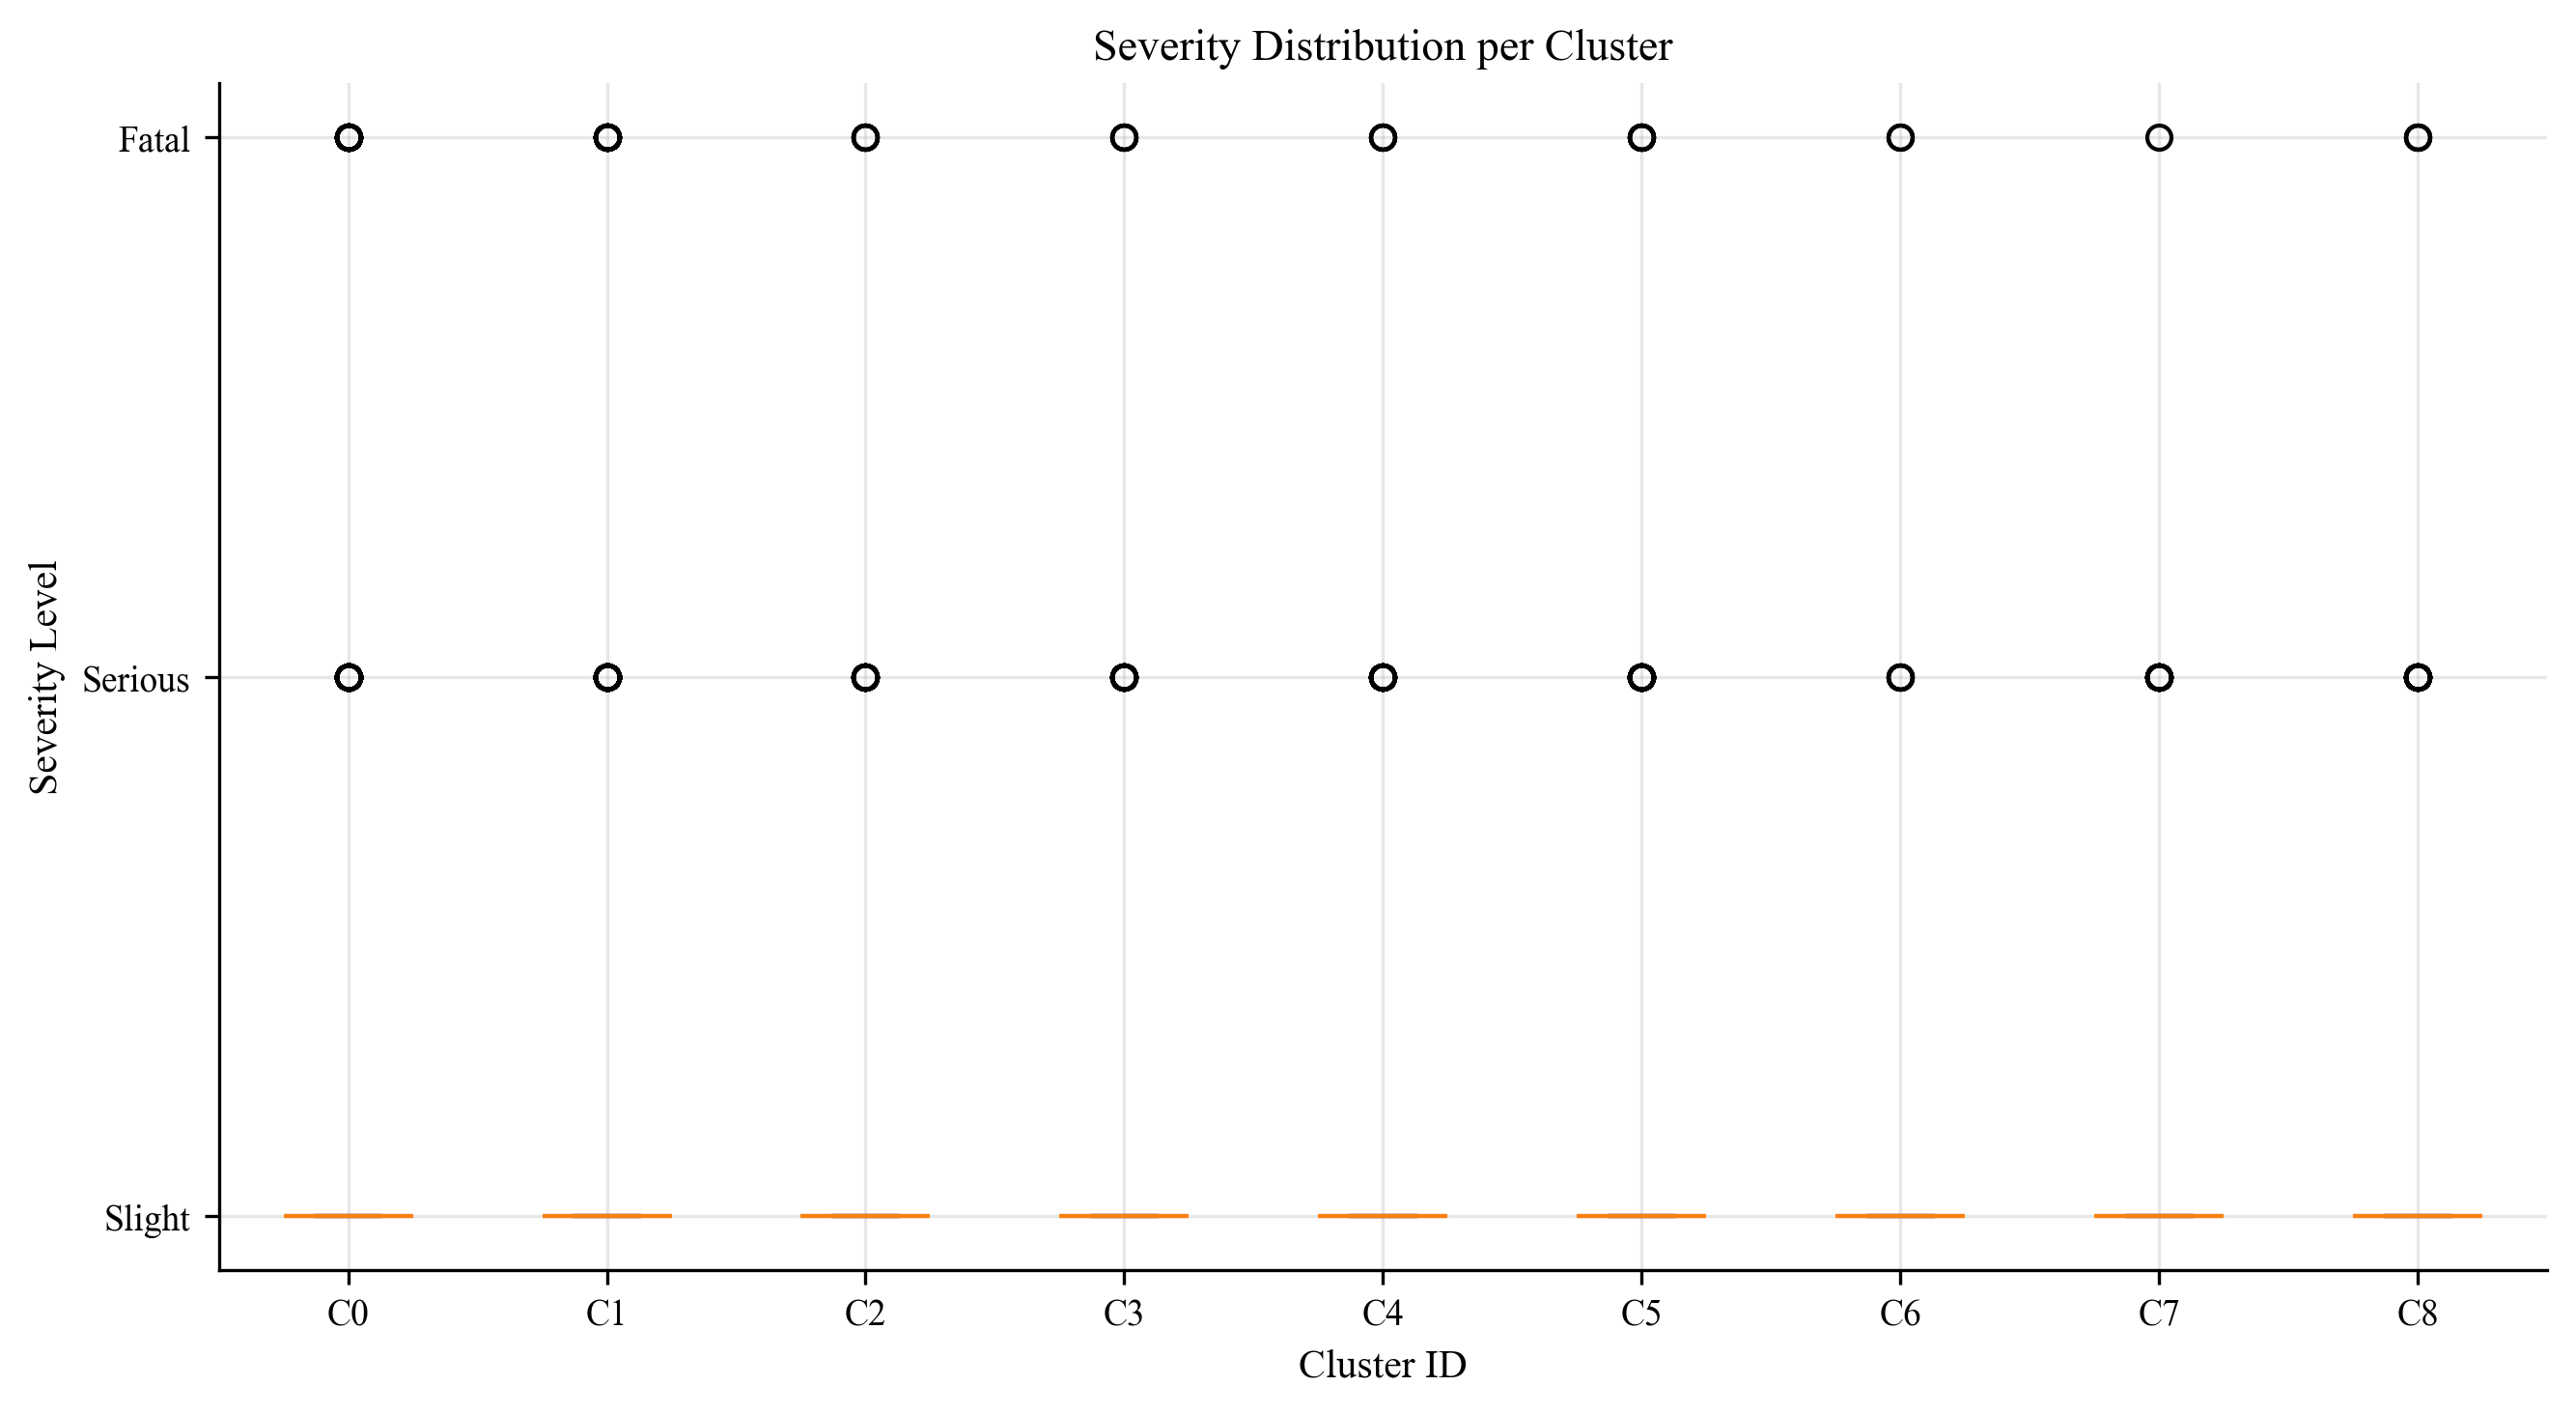
\includegraphics[width=\columnwidth]{figures/fig13_cluster_severity.png}}
\caption{Severity composition by cluster, showing the proportion of Slight, Serious, and Fatal injuries within each cluster.}
\label{fig:cluster_sev}
\end{figure}

\subsection{Discussion}

The system has a clear strength: DBSCAN finds geographically coherent clusters without pre-setting the number of regions, and the ARI turns those outputs into a priority list that is easier to act on than raw counts alone. Including Cluster\_ID in the classifier also adds measurable spatial context.

The major limitation is class imbalance. With 84.56\% of records belonging to the Slight Injury class, the classifier defaults to Slight for most inputs. Balanced class weighting helps, but not enough. Several factors contribute to this limitation:

\begin{enumerate}
\item The features in the dataset describe accident circumstances (weather, road type, junction type) but not crash dynamics (speed, impact angle, vehicle deformation). Severity is largely determined by crash dynamics, which are not available in police-report-style data.
\item Fatal injuries comprise only 158 records (1.28\%), which is too few for a tree-based ensemble to learn stable patterns from, even with class weighting.
\item The geocoding step maps categorical area types to city-level coordinates with jitter. This introduces spatial noise that may dilute the spatial signal available to the classifier.
\end{enumerate}

Even with that limitation, the system still offers a complete pipeline from raw data to a risk-tiered map, and the Flask API keeps the workflow usable from external applications.

\section{Conclusion and Future Work}

This paper presented an integrated accident hotspot prediction system that combines DBSCAN spatial clustering, Random Forest classification, and a data-driven ARI. On 12,316 Indian road accident records, DBSCAN identified 9 clusters and the Random Forest model reached 84.66\% test accuracy, with hour of day, cause of accident, and day of week emerging as the strongest predictors. The ARI then separated the clusters into two Severe, two Moderate, and five Low-risk groups.

At the same time, the classifier remains weak on minority classes. Cohen's Kappa of 0.0198 and a macro F1-score of 0.3149 show that Serious and Fatal injuries are not being separated reliably.

Several directions could improve future versions of the system:

\begin{enumerate}
\item \textbf{Oversampling techniques.} SMOTE or ADASYN could give the classifier more minority-class signal during training.

\item \textbf{Richer spatial data.} Replacing geocoded area labels with actual GPS coordinates would likely improve clustering quality and the usefulness of Cluster\_ID.

\item \textbf{Alternative models.} Models that encode spatial structure may capture interactions that tree-based methods miss.

\item \textbf{Real-time integration.} Live traffic and weather feeds could turn the current workflow into an early-warning system.

\item \textbf{Additional features.} Vehicle speed, hospital proximity, and emergency response time could improve severity prediction.

\item \textbf{Binary classification reformulation.} Collapsing the three severity classes into two may produce a more practical classifier by reducing the imbalance problem.
\end{enumerate}

The source code, trained models, and API are publicly available at the project repository.

\section*{Acknowledgment}

The authors thank Lovely Professional University for providing the computational resources and academic support for this research. The accident dataset was obtained from Kaggle, contributed by S3Programmer.

\begin{thebibliography}{00}

\bibitem{b1} World Health Organization, ``Global status report on road safety 2023,'' WHO, Geneva, Tech. Rep., 2023.

\bibitem{b2} Ministry of Road Transport and Highways, ``Road accidents in India -- 2022,'' Government of India, New Delhi, Annual Report, 2023.

\bibitem{b3} S. Mohan, ``Road traffic injuries and fatalities in India: time for action,'' \textit{Natl. Med. J. India}, vol. 35, no. 4, pp. 193--196, 2022.

\bibitem{b4} T. K. Anderson, ``Kernel density estimation and K-means clustering to profile road accident hotspots,'' \textit{Accid. Anal. Prev.}, vol. 41, no. 3, pp. 359--364, 2009.

\bibitem{b6} S. Kumar and D. Toshniwal, ``A data mining framework to analyze road accident data,'' \textit{J. Big Data}, vol. 2, no. 1, pp. 1--18, 2015.

\bibitem{b8} V. Prasannakumar, H. Vijith, R. Charutha, and N. Geetha, ``Spatio-temporal clustering of road accidents: GIS based analysis and assessment,'' \textit{Procedia Soc. Behav. Sci.}, vol. 21, pp. 317--325, 2011.

\bibitem{b9} M. Abdel-Aty and H. Abdelwahab, ``Predicting injury severity levels in traffic crashes: a modeling comparison,'' \textit{J. Transp. Eng.}, vol. 130, no. 2, pp. 204--210, 2004.

\bibitem{b10} L. Jiang, W. Xie, and B. Ren, ``Crash severity prediction using Random Forest and gradient boosting methods,'' in \textit{Proc. IEEE Int. Conf. Intell. Transp. Syst. (ITSC)}, 2020, pp. 1--6.

\bibitem{b11} F. Zong, H. Xu, and H. Zhang, ``Prediction for traffic accident severity: comparing the Bayesian network and regression models,'' \textit{Math. Probl. Eng.}, vol. 2013, pp. 1--9, 2013.

\bibitem{b14} N. V. Chawla, K. W. Bowyer, L. O. Hall, and W. P. Kegelmeyer, ``SMOTE: synthetic minority over-sampling technique,'' \textit{J. Artif. Intell. Res.}, vol. 16, pp. 321--357, 2002.

\bibitem{b16} J. Bao, P. Liu, and S. V. Ukkusuri, ``A spatiotemporal deep learning approach for citywide short-term crash risk prediction with multi-source data,'' \textit{Accid. Anal. Prev.}, vol. 122, pp. 239--254, 2019.

\bibitem{b18} A. Saha, S. Patil, and S. S. Joshi, ``Accident black spot identification on rural highways using GIS and weighted severity index,'' \textit{Int. J. Innov. Res. Sci. Eng. Technol.}, vol. 5, no. 6, pp. 10454--10461, 2016.

\bibitem{b19} S3Programmer, ``Road accident severity in India,'' Kaggle, 2023. [Online]. Available: https://www.kaggle.com/datasets/s3programmer/road-accident-severity-in-india

\bibitem{b20} M. Ester, H.-P. Kriegel, J. Sander, and X. Xu, ``A density-based algorithm for discovering clusters in large spatial databases with noise,'' in \textit{Proc. 2nd Int. Conf. Knowl. Discov. Data Min. (KDD)}, 1996, pp. 226--231.

\bibitem{b21} L. Breiman, ``Random forests,'' \textit{Mach. Learn.}, vol. 45, no. 1, pp. 5--32, 2001.

\end{thebibliography}

\end{document}
